\documentclass[12pt, twoside]{report}
\usepackage[utf8]{inputenc}
\usepackage[portuguese]{babel}
\usepackage[a4paper, top=30mm, left=20mm, bottom=20mm,
    right=20mm]{geometry}
\usepackage[dvipsnames]{xcolor}
\usepackage{graphicx}
\usepackage{color}
\usepackage{fancyhdr}
\fancyhead[LO,RE]{\itshape \nouppercase Chapter \arabic{chapter}}
\usepackage{amssymb}
\usepackage{csquotes}
\usepackage{amsmath}
\usepackage{amsthm}
\usepackage{faktor}
\usepackage[backend=bibtex, 
            maxbibnames=10,
            style=alphabetic]{biblatex}
\usepackage{hyperref}
\usepackage{subfigure}
\usepackage[font={small,it}]{caption}
\usepackage{algpseudocode}
\usepackage[plain]{algorithm}
\usepackage[shortlabels]{enumitem}

\pagestyle{fancy}

% Images path
\graphicspath{ {img/} }

% ABNT foreign words should be in italic
\newcommand{\foreignword}[1]{\textit{#1}}
\newcommand{\toolname}[1]{\textit{#1}}
\newcommand{\fieldR}{\mathbb{R}}
\newcommand{\powerset}{\mathcal{P}}
\newcommand{\probability}{\mathbb{P}}
\newcommand{\expectation}{\mathbb{E}}
\newcommand{\algname}[1]{\texttt{#1}}
\newcommand{\langname}[1]{\texttt{#1}}
\newcommand{\varname}[1]{\texttt{#1}}
\newcommand{\floor}[1]{\lfloor #1 \rfloor}
\newcommand{\ceil}[1]{\lceil #1 \rceil}
\newcommand{\mathsc}[1]{{\normalfont\textsc{#1}}}
\newcommand{\forest}{\mathcal{F}}
\newcommand{\pfsnode}[1]{\mathbf #1}

\algrenewcommand\Return{\State \algorithmicreturn{} } % tirar os returns da mesma linha nos pseudocodigos 


\DeclareMathOperator*{\argmin}{argmin} 

\addbibresource{references.bib}

\newtheorem{mydefinition}{Definição}
\numberwithin{mydefinition}{section}
\newtheorem{mytheorem}{Teorema}
\numberwithin{mytheorem}{section}
\newtheorem{mylemma}{Lema}
\numberwithin{mylemma}{section}


% TODO: 
% incluir featsel nas referências

\begin{document}


\pagenumbering{roman}
\thispagestyle{empty}
\begin{center}
{\Large
{\bf Projeto de Algoritmos Baseados em Florestas de Posets para o 
     Problema de Otimização U-curve}\\
\bigskip
\bigskip
\bigskip
\textsc{
    Monografia apresentada\\[-0.25cm] 
    ao\\[-0.25cm]
    Instituto de Matemática e Estatística\\[-0.25cm]
    da\\[-0.25cm]
    Universidade de São Paulo\\[-0.25cm]
    para\\[-0.25cm]
    aprovação em MAC499 -- Trabalho\\[-0.25cm]
    de\\[-0.25cm]
    Conclusão de Curso}\\
\bigskip
\bigskip
\bigskip
{\bf Aluno:} \href{mailto:gustavo.estrela.matos@gmail.com}{Gustavo Estrela de Matos}\\
\bigskip
{\bf Orientador:} \href{mailto:marcelo.reis@butantan.gov.br}{Marcelo da Silva Reis}\\
\bigskip
\bigskip
\bigskip
Centro de Toxinas, Resposta-imune e Sinalização Celular (CeTICS)\\
\bigskip
Laboratório Especial de Ciclo Celular, Instituto Butantan\\
\bigskip
\bigskip
\bigskip
São Paulo, \today
}
\end{center}
\newpage

\chapter*{Resumo}
A fazer.
%O problema U-curve é uma formulação de um problema de otimização que 
%pode ser utilizado na etapa de seleção de características em Aprendizado
%de Máquina, com aplicações em desenho de modelos computacionais de 
%sistemas biológicos. Não obstante, soluções propostas até o presente 
%momento para atacar esse problema têm limitações do ponto de vista de 
%consumo de tempo computacional e/ou de memória, o que implica na 
%necessidade do desenvolvimento de novos algoritmos. Nesse sentido, em 
%2012 foi proposto o algoritmo Poset-Forest-Search (PFS), que organiza o
%espaço de busca em florestas de posets. Esse algoritmo foi implementado 
%e testado, com resultados promissores; todavia, novos melhoramentos são
%necessários para que o PFS se torne uma alternativa competitiva para 
%resolver o problema U-curve. Neste projeto propomos a construção de uma 
%versão paralelizada e escalável do algoritmo PFS, utilizando diagramas 
%de decisão binária reduzidos e ordenados. Além disso, propomos adaptar 
%o PFS como um algoritmo de aproximação, no qual o critério de 
%aproximação da solução ótima faça uso do teorema da navalha de Ockham. 
%Os algoritmos desenvolvidos serão implementados e testados em instâncias
%artificiais e também em conjuntos de dados próprios para experimentos 
%comparativos entre diferentes algoritmos de seleção de características.

\tableofcontents

\clearpage
\pagenumbering{arabic} 

\nocite{*}
\chapter{Introdução}
% - machine learning e seleção de características
%    problema: falta de amostras
%    solução: simplificar o modelo de aprendizado -> seleção de 
%             características    
% - problema de otimização
% - funções de custo
% - aplicações: w-operadores, construção de modelos funcionais
% - algoritmos de seleção de características
% - trabalhos antigos

Seleção de características é uma técnica que pode ser utilizada em uma das
etapas da construção de um modelo de aprendizado de máquina. Ela consiste
em, dado o conjunto de características observadas nas amostras, escolher
um subconjunto que seja ótimo de acordo com alguma métrica. Devemos 
considerar o uso de seleção de características quando a quantidade de
características é muito grande, o que pode tornar o uso do modelo muito caro
do ponto de vista computacional. Outra aplicação dessa técnica é em situações
nas quais a quantidade de amostras é pequena comparada à complexidade do 
modelo original, em outras palavras, quando ocorre sobreajuste (do 
inglês, \foreignword{overfitting}).

Mais formalmente, o problema de seleção de características consiste em
um problema de otimização combinatória em que, dado um conjunto $S$ de 
características, procuramos por um subconjunto $X \in \powerset (S)$
ótimo de acordo com uma função de custo $c : \mathcal{P}(S) \to 
\fieldR_{+}$. {\color{blue}É comum nas abordagens do problema explorar o fato de que
o espaço de busca $\powerset(S)$ junto a relação $\subseteq$ define um
reticulado Booleano {\bf[Adicionar referência(s) para esta afirmação]}}. No geral, a função de custo $c$ deve ser capaz de
medir quão informativas as características $X$ são em respeito ao rótulo
$Y$ do problema de aprendizado; portanto $c$ costuma depender da
estimação da distribuição de probabilidade conjunta de $(X, Y)$.

Quando ocorre a estimação da distribuição de probabilidade conjunta de 
$(X, Y)$, o custo das cadeias do reticulado Booleano reproduzem um
fenômeno conhecido em aprendizado de máquina, o das ``curvas em U''. Para 
entender intuitivamente esse fenômeno, devemos observar que conforme 
subimos uma cadeia do reticulado estamos aumentando o número de 
características sendo consideradas, portanto existem mais possíveis
valores de $X$, permitindo descrever melhor os valores de $Y$; por outro
lado, também precisaríamos de mais amostras para estimar bem 
$\probability (X, Y)$, e, quando isso não é possível, erros de estimação
fazem com que $c(X)$, isto é, o custo de $X$, aumente.

Podemos então considerar um caso particular do problema de seleção de
características em que a função de custo descreve ``curvas em U''
em todas as cadeias do reticulado Booleano. Esse caso particular é 
conhecido como problema U-curve e existem na literatura algoritmos 
ótimos para esse problema como o \algname {U-Curve Branch and Bound 
(UBB), U-Curve-Search (UCS) e Poset Forest Search (PFS)} {\color{blue}[Adicionar referências para os algoritmos]}. A solução do 
problema U-curve tem aplicações em problemas de aprendizado de máquina tais como como projeto
de W-operadores~\cite{MJCJJB} e preditores na estimação de Redes Gênicas 
Probabilísticas~\cite{BCJMJ07}.

O problema U-Curve é NP-difícil~\cite{REI12}; por conta deste fato, os algoritmos 
apresentados até então na literatura têm limitações tanto do ponto de vista de
tempo de computação quanto do uso de memória. Dentre estes algoritmos,
destacamos o PFS, que foi criado como um melhoramento do algoritmo UBB. 
O algoritmo PFS organiza o reticulado Booleano $(\mathcal{P}(S),\subseteq)$ em uma floresta de posets, composta de árvores disjuntas que são subgrafos da árvore que constitui o espaço de busca do algoritmo UBB. Além disso, PFS também mantém uma floresta de posets composta de árvores induzidas a partir de uma árvore construída a partir do reticulado Booleano dual $(\mathcal{P}(S),\supseteq)$. Uma vez que o espaço de busca é composto de várias árvores disjuntas, parece razoável a hipótese de que a paralelização 
desse algoritmo possa trazer ganhos do ponto de vista de consumo de 
tempo. Além disso, a escolha de árvores para etapa de ramificação no 
algoritmo também pode ser explorada e pode trazer ganhos em respeito ao
consumo de tempo e de memória.

{\color{blue}[Comentário: acho que vai ter que revisar a explicação básica da dinâmica do PFS, detalhando-a mais e/ou fazendo referências para minha tese. Uma ideia seria aproveitar o que escrevemos sobre o PFS no projeto de mestrado]}.

\section{Objetivos do Trabalho}
Podemos dividir os objetivos deste trabalho em objetivos gerais e 
específicos.\\

{\bf Objetivos gerais}:
\begin{enumerate}
\item{Criar algoritmos para o problema U-curve que sejam mais eficientes
em consumo de tempo e/ou de memória do que as presentes soluções;}
\item{Verificar a qualidade das soluções encontradas no desenvolvimento
de modelos de Aprendizado Computacional.}
\end{enumerate}

{\bf Objetivos específicos}:
\begin{itemize}
\item{Estudar o algoritmo \algname {Poset Forest Search (PFS)};}
\item{Modificar a etapa de ramificação do algoritmo \algname{PFS} e avaliar
as mudanças na dinâmica do algoritmo;}
\item{Paralelizar o algoritmo \algname{PFS}, com as modificações feitas
na etapa de ramificação (se houver melhorias com tal mudança);}
\item{Criar um novo algoritmo, de natureza paralela e facilmente combinável com outros algoritmos, para o problema 
U-Curve (o algoritmo \algname{PUCS});}
\item{Avaliar o consumo de recursos computacionais dos algoritmos 
criados, comparando com os algoritmos já presentes na literatura como
o \algname{UBB};}
\item{Avaliar os conjuntos de características selecionados por cada 
algoritmo na seleção de modelos de aprendizado computacional, usando 
como exemplo conjuntos de dados do repositório \href{https://archive.ics.uci.edu/ml/index.php}{UCI Machine Learning 
Repository.}}
\end{itemize}

\section{Organização do Trabalho}

A fazer, resumo de cada capítulo da monografia.



\chapter{Conceitos Fundamentais}
% Contextualização e conceitos fundamentais
% .1 O problema de seleção de características
% .2 Funções de custo para esse problema
% .3 Redução para o problema de curvas em U

\section{O problema de seleção de características}
A seleção de características é um problema de otimização combinatória 
em que procuramos o melhor subconjunto de um conjunto de características
$S$. O espaço de busca desse problema é o conjunto potência de $S$, 
$\powerset (S)$, que é a coleção de todos os subconjuntos possíveis de
 $S$. A função de custo desse problema é uma função $c : \powerset (S) 
\to \fieldR_{+}$.

\begin{mydefinition}[Problema de seleção de características] Seja $S$
um conjunto de características, finito e não vazio, e $c$ uma função de 
custo. Encontrar $X \in \powerset (S)$ tal que $c (X) \leq c (Y)$,
$\forall Y \in \powerset (S)$.
\end{mydefinition}

O espaço de busca do problema de seleção de características possui uma
relação de ordem parcial definida pela relação $\subseteq$, portanto
este conjunto é {\bf parcialmente ordenado (poset)}.

\begin{mydefinition}
Uma {\bf \em cadeia} do reticulado booleano é uma sequência $X_1$, 
$X_2$, ..., $X_l$ tal que $X_1 \subseteq X_2 \subseteq \dots 
\subseteq X_l$.
\end{mydefinition}


%No contexto de aprendizado de máquina, é comum que as funções de custo
%utilizadas na seleção de característica descrevam curvas próximas do 
%formato de u nas cadeias do reticulado. Esse fenômeno é conhecido em 
%aprendizado e explicaremos como ele ocorre na seção 
%\ref{fund_concept:cost_functions}.

\section{Funções de custo}
Nesta seção apresentaremos as duas funções de custo mais utilizadas 
durante este trabalho: a entropia condicional média (MCE) e a soma de 
subconjuntos. A primeira foi utilizada na seleção de modelos de
aprendizado, enquanto a segunda foi utilizada para criação e solução
de instâncias artificiais. 
%A função de soma de subconjuntos é 
%decomponível em curvas u e a MCE não, porém explicaremos como a última 
%função deve ter um formato parecido com a da curva em u.

\subsection{Custo de modelos de aprendizado computacional} 
\label{fund_concept:cost_functions} A função de custo utilizada na 
solução do problema deve, de alguma forma, refletir a qualidade do 
conjunto de características avaliado. Por isso,
diferentes aplicações de seleção de características
podem ter diferentes funções de custo. No contexto de aprendizado de 
máquina, uma possível função de custo é a entropia condicional média
(MCE), que já foi utilizada por exemplo na construção de W-operadores
~\cite{MJCJB06}.

\begin{mydefinition}\label{def:conditional_entropy}
Dado um problema de aprendizado em que $Y$ é o conjunto de possíveis
rótulos e $W = (w_1, ..., w_n)$, com $w_i \in A_i$, é o conjunto de
variáveis. Seja $W' = (w_{I(1)}, w_{I(2)}, ..., w_{I(k)})$ um conjunto 
de variáveis (características) escolhidas, $\mathbf{X}$ uma vetor 
aleatório de tamanho $k$ com ${X_j} \in A_{I(j)}$, e $log0 = 0$. Então,
a {\bf \em entropia condicional} de $Y$ dado $\mathbf{X} = \mathbf x$ é:

\begin{center}
$
\begin{aligned}
H (Y | \mathbf{X = x}) = - 
\sum_{y \in Y} \probability (Y = y | \mathbf{X = x}) log \probability (Y = y | \mathbf{X = x})
\end{aligned}
$
\end{center}
\end{mydefinition}

\begin{mydefinition}
Sob o mesmo contexto definido em \ref{def:conditional_entropy}, 
definimos a {\bf \em entropia condicional média} como:
\begin{center}
$
\begin{aligned}
    \expectation[H (Y | \mathbf{X})] = 
    \sum_{\mathbf{x} \in \mathbf{X}} H (Y | \mathbf{X = x}) \probability (\mathbf{X = x})
\end{aligned}
$
\end{center}
\end{mydefinition}

%Vamos usar esta função como exemplo para entender intuitivamente como
%as funções de custo no problema de seleção de características descrevem
%curvas em u.

A função $H$, em teoria da informação, mede o inverso da quantidade 
média de informação que uma variável tem. Esta função atinge valor 
máximo quando a distribuição de probabilidade da variável aleatória em
questão é uniforme (todos valores que ela pode assumir são 
equiprováveis), e tem valores baixos quando essa distribuição é 
concentrada. 

Problemas de aprendizado em que os rótulos tem uma distribuição 
concentrada são mais fáceis do que os problemas em que essa distribuição
é menos concentrada. Tome como exemplo o problema de
classificar o lançamento de uma moeda $\mathbf{x}$ em $y$ (cara ou 
coroa); se toda moeda $\mathbf{x}$ é não viciada, então a distribuição
de $\probability (y | \mathbf{x})$ é pouco concentrada, por outro lado,
quando a moeda é viciada, a distribuição de 
$\probability (y | \mathbf{x})$ é concentrada e é mais fácil 
classificar este problema. Em termos mais formais, o erro do melhor 
classificador do problema mais fácil é menor do que o erro do melhor 
classificador do problema mais difícil.

Portanto, como a função $H$ é capaz de medir a concentração da 
distribuição de $Y$ dado $\mathbf{X = x}$, e quanto maior esta 
concentração mais fácil é o modelo de aprendizado, podemos  dizer
que a função de custo $\expectation[H (Y | \mathbf{X = x})]$ pode 
representar a qualidade do modelo de classificação que usa o conjunto de
características de $\mathbf{X}$.

Agora, como já entendemos o funcionamento da função de custo
MCE e como ela se relaciona com a qualidade do conjunto de 
características avaliado, vamos entender o que acontece no modelo de 
aprendizado e na função de custo que usamos como exemplo quando 
percorremos uma cadeia do reticulado. 

Uma cadeia do poset pode ser vista como uma sequência de possíveis
escolhas de conjuntos de características ao qual a cada passo 
adicionamos uma característica. Isso significa que a cada passo dado
a variável $\mathbf{x}$ ganha uma componente a mais. Quando estamos no 
início da cadeia, poucas variáveis do problema são consideradas, 
portanto há uma grande abstração dos dados dos objetos sendo 
classificados, e conforme subimos uma cadeia, diminuímos a abstração dos
dados e isso faz com que a distribuição de $Y$ dado $\mathbf{x}$ se 
concentre.

Essa concentração da distribuição da probabilidade indica que o custo 
dos subconjuntos deve diminuir conforme subimos por uma cadeia do 
reticulado, ou seja, este raciocínio nos leva a pensar que adicionar 
características sempre melhora a classificação; de fato, o valor de
$\expectation[H (Y | \mathbf{X = x})]$ deve diminuir (até algum ponto 
de saturação) conforme aumentamos o número de variáveis do problema. 
Mas se isso é verdade, por que fazemos seleção de características? A 
inconsistência entre esse raciocínio e a motivação para seleção de 
característica é que essa linha de raciocínio negligenciou que problemas
de classificação (supervisada) dependem de uma amostra da distribuição 
de $Y$ dado $\mathbf{X = x}$, ou seja, não sabemos nem ao menos calcular
$H (Y | \mathbf{X = x})$, podemos apenas estimar o seu valor a partir
da amostra.

A amostra da distribuição de $Y$ dado $\mathbf{X = x}$ é obtida do 
conjunto de treinamento do problema de aprendizado e quando o número
de amostras não é grande o suficiente a qualidade do classificador 
é comprometida. Além disso, o número de amostras necessárias deve
crescer conforme aumentamos a complexidade do modelo de aprendizado 
utilizado. Considerando que quando subimos uma cadeia do reticulado 
booleano estamos aumentando a complexidade do modelo, temos que, a
partir de um certo ponto, a qualidade do classificador que utiliza tal 
conjunto de características deve piorar. 

Portanto, é esperado que a função de custo descreva um formato de u nas 
cadeias do reticulado. No começo da cadeia, o custo deve diminuir por 
conta da maior granularidade dos dados de entrada, até algum ponto onde
a limitação no número de amostras combinada com o aumento da 
complexidade do modelo causem erros de estimação que aumentam o erro
do classificador criado em tal modelo.

No cálculo da entropia condicional média, o efeito do aumento da 
complexidade de $\mathbf X$ é a estimação ruim de 
$\probability (Y = y | \mathbf{X = x})$. Contorna-se este problema 
modificando a entropia condicional média para penalizar a entropia de 
$Y$ quando $\mathbf{x}$ foi observado poucas vezes. A função de custo
utilizada é, então:

\begin{center}
$
\begin{aligned}
    \hat{\expectation}[H (Y | \mathbf{X})] = \frac{N}{t}
    \sum_{\mathbf{x} \in \mathbf{X}} H (Y | \mathbf{X = x}) \probability (\mathbf{X = x})
\end{aligned}
$
\end{center}

\subsection{Soma de subconjuntos}
Para se avaliar o desempenho dos algoritmos criados neste trabalho, 
utilizamos instâncias artificiais que são reduções do problema da soma
de subconjuntos. Este problema consiste em, dado um conjunto finito de
inteiros não-negativos $S$ e um inteiro não-negativo $t$, descobrir se
há um subconjunto de $S$ que soma $t$. Podemos resolver este problema 
com a solução de uma instância do problema de seleção de características
onde o conjunto de características é $S'$ uma cópia de $S$ e a função de
custo é $c$:

\begin{equation*} \label{cost_function:subset_sum}
    c (X) = |t - \sum_{x \in X} x| \text{, para todo } 
                                        X \in \powerset(S') \text{.}
\end{equation*}

Assim como a função de custo MCE, a função de custo de somas de 
subconjuntos também apresenta um formato interessante nas cadeias
do reticulado booleano. Para toda cadeia com elementos $A \subseteq B 
\subseteq C$ vale que $c (B) \leq max\{c (A), c (B)\}$. Vamos provar 
esta propriedade para dois casos disjuntos, quando $|t - \sum_{b \in B}
b| > 0$ e quando $|t - \sum_{b \in B} b| \leq 0$. Começamos a 
demonstração definindo $D = B \setminus A$ e $E = C \setminus B$.

\begin{itemize}
    \item{se $|t - \sum_{b \in B} b| > 0$, então:}
    \begin{align*}
        c (B) & =  |t - \sum_{b \in B} b|  & \\
              & \leq  |t - \sum_{b \in B} b + \sum_{d \in D} d| & 
                \text{(pois $S$ contém apenas números positivos e $t -
                \sum_{b \in B} b > 0$)} \\
              & = |t - \sum_{a \in B \setminus D} a| \\
              & = |t - \sum_{a \in A} a| \\
              & = c (A)
    \end{align*}
    portanto, $c (B) \leq  c (A)$, logo $c (B) \leq max \{c (A), c (C)\}$.
    
    \item{se $|t - \sum_{b \in B} b| \leq 0$, então:}
    \begin{align*}
        c (B) & =  |t - \sum_{b \in B} b|  & \\
              & \leq  |t - \sum_{b \in B} b - \sum_{e \in E} e| & 
                \text{(pois $S$ contém apenas números positivos e $t -
                \sum_{b \in B} b \leq 0$)} \\
              & = |t - \sum_{c \in B \cup E} c| \\
              & = |t - \sum_{c \in C} c| \\
              & = c (C)
    \end{align*}
    portanto, $c (B) \leq  c (C)$, logo $c (B) \leq max \{c (A), c (C)\}$.
\end{itemize}
Como acabamos de provar para os dois casos possíveis, temos que 
$c (B) \leq max \{c (A), c (C)\}$. \qed

\section{O problema U-Curve}
As duas funções de custo apresentadas na seção ~\ref{fund_concept:cost_functions}
descrevem curvas que tem um formato em U (a menos de oscilações) nas 
cadeias do reticulado booleano, vamos definir esta propriedade agora.

\begin{mydefinition}
Uma cadeia é dita {\bf \em maximal} se não existe outra cadeia no 
reticulado que contenha propriamente esta cadeia.
\end{mydefinition}

\begin{mydefinition}\label{fund_concepts:ushape}
Uma função de custo $c$ é dita {\bf \em decomponível em curvas U} se
para toda cadeia maximal $X_1, ..., X_l$, $c(X_j) \leq max \{c (X_i),
c (X_k)\}$ sempre que $X_i \subseteq X_j \subseteq X_k$, $i, j, k \in 
\{1, ..., l\}$.
\end{mydefinition}

Vamos considerar então o problema de seleção de características em que a
função de custo utilizada é decomponível em curvas U. Este é o problema 
central deste trabalho.

\begin{mydefinition}[Problema U-Curve]
Dados um conjunto finito e não-vazio $S$ e uma função de custo $c$ 
decomponível em curvas em U, encontrar um subconjunto $X \in 
\powerset (S)$ tal que $c(X) \leq c(Y)$,  $\forall Y \in \powerset (S)$.
\end{mydefinition}

O problema U-Curve é um caso particular do problema de seleção de 
características com uma propriedade que nos permite achar o mínimo
global sem a necessidade de avaliar cada ponto do reticulado booleano. 
Isso é possível porque a propriedade U-Curve (da decomponibilidade da 
função de custo em curvas U) nos garante que o custo dos elementos de 
uma cadeia não podem cair uma vez que aumentaram. Sejam por exemplo
dois elementos $A \subseteq B$ de $\powerset (S)$, então:
\begin{itemize}
    \item{se $c(B) > c (A)$, então $c (X) > c (A)$ para todo $X$
        do intervalo $[B, \powerset (S)]$;}
    \item{se $c(A) > c (B)$, então $c (X) > c (B)$ para todo $X$ 
        do intervalo $[\emptyset, A]$;}
\end{itemize}

Desta maneira, quando um problema de seleção de características tem uma 
função de custo decomponível em curvas U a menos de algumas oscilações,
é vantajoso aproximar a solução deste problema pela solução encontrada
por um algoritmo de busca do problema U-Curve. Tal abordagem não é 
ótima, porém, como existem poucas oscilações da função de custo, é 
provável que a solução encontrada ainda seja próxima da melhor solução.



\chapter{Melhoramentos no Poset Forest Search}
Neste capítulo apresentamos o algoritmo \algname{Poset-Forest-Search} 
(\algname{PFS}), um algoritmo ótimo para o problema U-curve que foi 
criado para enfrentar a limitação do algoritmo \algname{U-curve Branch 
and Bound} (\algname{UBB}) ser unidirecional. Apesar do \algname{PFS}
ter solucionado tal problema com sucesso, este algoritmo apresenta 
pontos que ainda podem ser explorados para se criar uma modificação que
tenha melhor desempenho computacional. Modificaremos então o 
\algname{PFS}, explorando tais pontos e, além disso, vamos criar uma
versão paralela do algoritmo.

Baseamos nosso trabalho no código-fonte do arcabouço featsel~\cite{Reis+17}, que é software 
livre e \href{https://github.com/msreis/featsel}{está disponível no GitHub} sob a licença de uso \foreignword{GNU General Public License}. Todos os experimentos computacionais deste capítulo foram feitos utilizando algoritmos e funções de custo implementados no featsel, em uma servidora com 64 núcleos, 256 GB de memória RAM e sistema operacional Ubuntu server 14.04 LTS. Em todos os experimentos foi utilizada como função de custo a redução polinomial do problema da soma de subconjuntos (equação~\ref{cost_function:subset_sum}); instâncias artificiais foram geradas escolhendo aleatoriamente $n + 1$ números inteiros, onde $n$ é o número de características.

\section{Descrição do algoritmo}
% - apresentar o UBB
%   - organização do espaço de busca em uma árvore
%   - pilha de busca em profundidade -> simples poda: não inserir nó
%     na pilha 
%   - limitação por ser unidirecional
% - apresentar o PFS
%   - duas florestas
%     - é bom explicar o que é leftmost aqui
%   - regras do jogo
%   - pseudo-código com as duas etapas
%   - indicar quais são os pontos que podem ser explorados

\subsection{O caso simples: o algoritmo \algname{U-curve-Branch-and-Bound} (\algname{UBB})}
O algoritmo \algname{U-curve Branch and Bound} (\algname{UBB}), que é 
uma versão simplificada do \algname{PFS}, percorre o espaço de busca 
fazendo uma busca em profundidade em uma árvore que é subgrafo do 
diagrama de Hasse do reticulado Booleano ($\powerset (S), \subseteq$). 
Esta árvore é definida por aplicações recursivas do seguinte lema:

\begin{mylemma}
\label{lemma:lower_forest}
Sejam $X$ e $Y$ conjuntos, $X$ não-vazio e $x_i$ o $i$-ésimo 
elemento de $X$. Seja $X_0 \supseteq X_1 \supseteq \dots \supseteq 
X_{|X|}$ uma cadeia tal que $X_0 = X$, $X_{|X|} = \emptyset$ e $X_{i} 
\cup \{x_i\} = X_{i - 1}$ para todo $0 < i \leq |X|$. Vale que:
\begin{align*}
\{ Y \} \cup \bigcup_{i = 1}^{|X|} \{W \cup Y \cup \{x_i\} : W \in \powerset (X_i)\} = \{W \cup Y : W \in \powerset (X)\}.
\end{align*}
\end{mylemma} 

\begin{proof}
Faremos uma prova por indução no tamanho de $X$ de maneira similar a
Reis ~\cite{Rei12}.

\begin{itemize}
\item{Suponha que $|X| = 1$. Então:}
\begin{align*}
    \{Y\} \cup \bigcup_{i = 1}^{1} \{W \cup Y \cup \{x_i\} : W \in \powerset (X_i)\} & = 
    \{Y\} \cup \{W \cup Y \cup \{x_1\} : W \in \powerset (X_1)\} & \\
    & = \{Y\} \cup \{Y \cup \{x_1\}\} \tag{Como $X_1 = \emptyset$} \\
    & = \{Y, Y \cup \{x_1\}\} \\
    & = \{W \cup Y : W \in \powerset (X)\}.
\end{align*}

\item{Suponha que o lema é verdadeiro para todo $X$ com $|X| < k$, 
    então:}
\begin{align*}
    & \{Y\} \cup \bigcup_{i = 1}^{k} \{W \cup Y \cup \{x_i\} : W \in \powerset (X_i)\} = \\
    & \{Y\} \cup \bigcup_{i = 2}^{k} \{W \cup Y \cup \{x_i\} : W \in \powerset (X_i)\} \cup \{W \cup Y \cup \{x_1\} : W \in \powerset (X_1) \}.
\end{align*}
Seja $Z = Z_0 = X_1, Z_1 = X_2, \dots Z_{|Z|} = X_{|X|}$, então
$|Z| = k - 1$ e $z_1 = x_2, z_2 = x_3, \dots, z_{|Z|} = x_{|X|}$, e:
\begin{align*}
    & \{Y\} \cup \bigcup_{i = 2}^{k} \{W \cup Y \cup \{x_i\} : W \in \powerset (X_i)\} \cup \{W \cup Y \cup \{x_1\} : W \in \powerset (X_1) \} =\\
    & \{Y\} \cup \bigcup_{j = 1}^{k - 1} \{W \cup Y \cup \{z_j\} : W \in \powerset (Z_i)\} \cup \{W \cup Y \cup \{x_1\} : W \in \powerset (X_1) \} =\\
    \tag{Pela hipótese de indução}  \\ 
    & \{Y \cup W : W \in \powerset (Z)\} \cup \{W \cup Y \cup \{x_1\} : W \in \powerset (X_1) \} =  \\
    & \{Y \cup W : W \in \powerset (X_1)\} \cup \{W \cup Y \cup \{x_1\} : W \in \powerset (X_1) \} =  \\
    & \{Y \cup W : W \in \powerset (X_1 \cup {x_1})\} = \\
    & \{Y \cup W : W \in \powerset (X)\}.
\end{align*}
\end{itemize}
\end{proof}

Para representar o espaço de busca como uma árvore, devemos aplicar o
lema da seguinte forma. Vamos utilizar o conjunto $X_Y$ para determinar 
para cada nó $Y$ do reticulado quais são os nós alcançáveis por ele, de
maneira que um nó $Y$ pode alcançar todo nó do intervalo 
$[Y, X_Y \cup Y]$. Iniciamos a construção da árvore com a base da 
aplicação recursiva do lema, indicando que $X_{Y = \emptyset} = S$, 
pois $\emptyset$ deve ser a raiz da árvore e deve alcançar qualquer 
outro nó. Agora suponha que estamos em um nó $Y$, então
definimos $X_0 = X_Y$, $X_{Y_i} \cup \{x_i\} = X_{Y_{i - 1}}$, e 
$Y_i = Y \cup \{x_i\}$ para $x_i \in X_Y$; então para criar a sub-árvore 
com raiz $Y$ basta adicionar os arcos $(Y, Y_i)$ para cada $i$ e aplicar 
o lema recursivamente para cada $Y_i$ e $X_{Y_i}$. A figura~\ref{fig:pfs:ubb_tree} mostra uma árvore arbitrária gerada pela 
aplicação recursiva do lema. 

\begin{figure}[!ht]
  \centering 
  \begin{tabular}{c c}
    \subfigure[] {\scalebox{0.4}{
     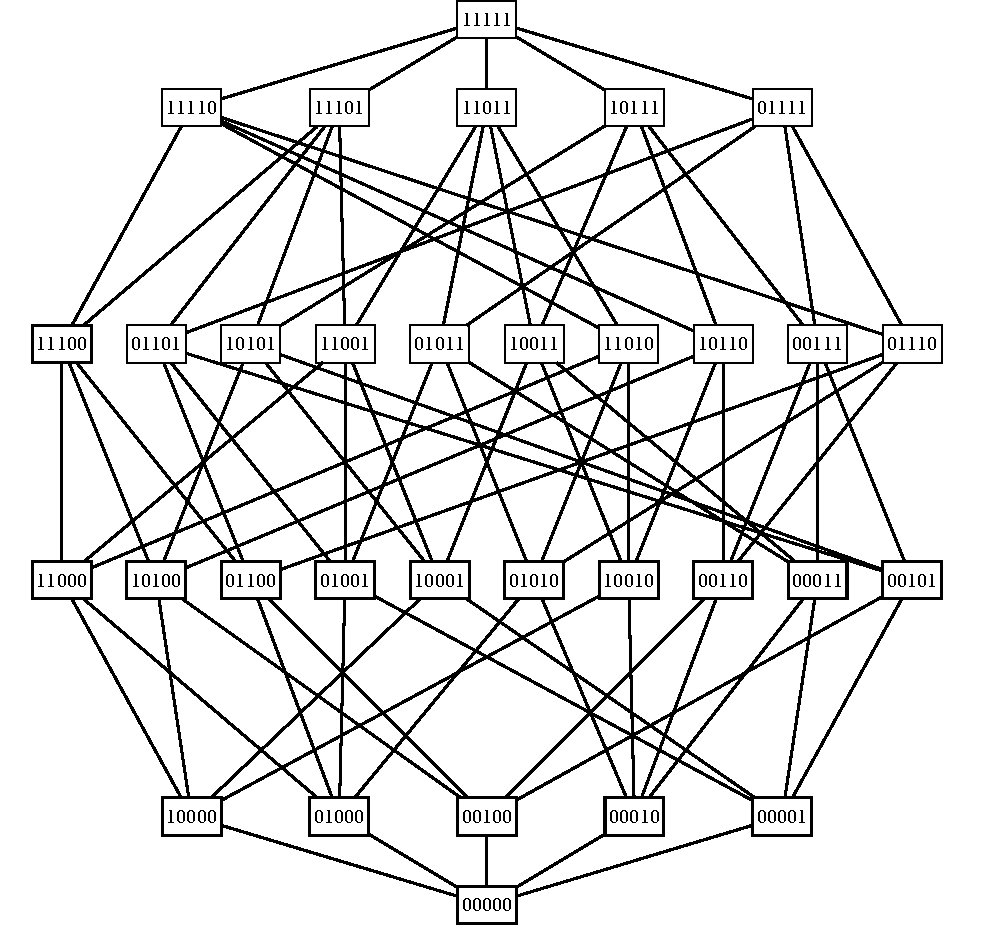
\includegraphics[clip=true]{pfs/ubb/full_lattice.pdf}}
     \label{fig:ubb:full} }
    & 
    \subfigure[] {\scalebox{.4}{
    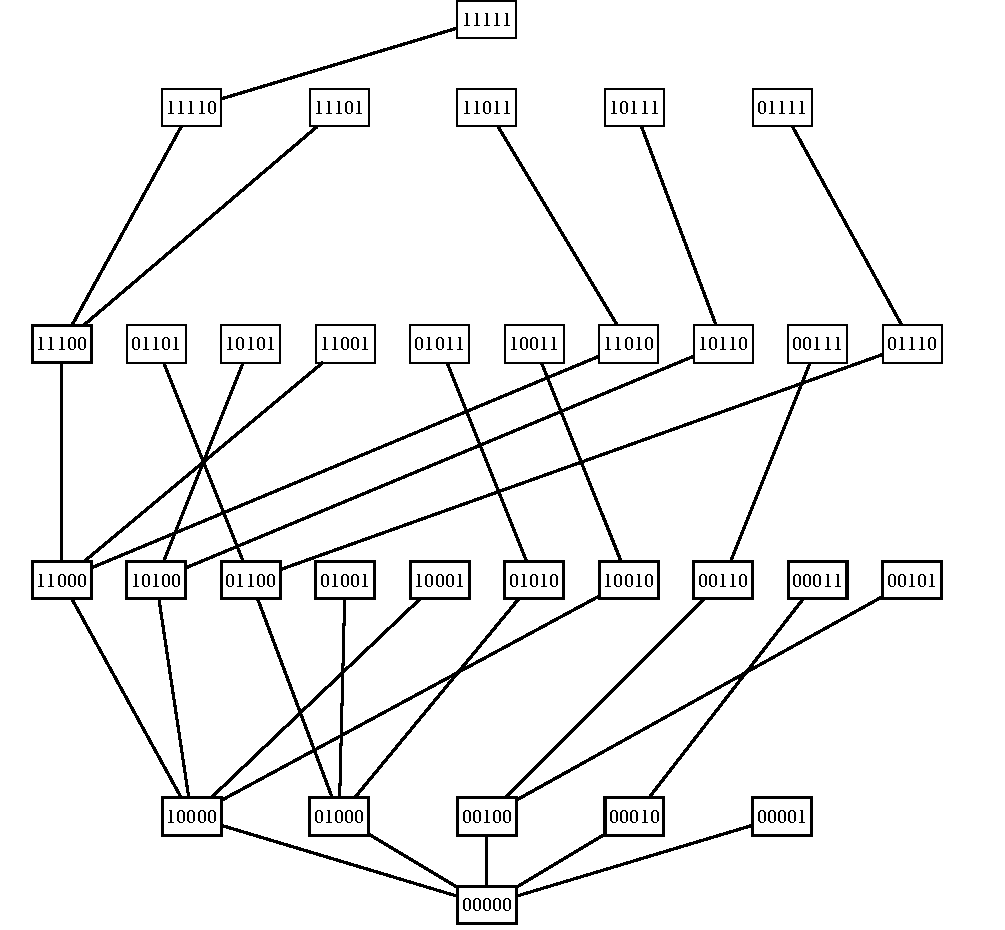
\includegraphics[clip=true]{pfs/ubb/ubb_tree.pdf}}
    \label{fig:ubb:tree} }
  \end{tabular}
    \caption{A figura ~\ref{fig:ubb:full} é o diagrama de Hasse do
    reticulado Booleano ($\powerset (S), \subseteq$) e a figura
    ~\ref{fig:ubb:tree} é uma árvore de busca definida pelo algoritmo
    \algname{UBB}.}
  \label{fig:pfs:ubb_tree} 
\end{figure}

A dinâmica do \algname{UBB} é simples. Aplica-se o lema 
~\ref{lemma:lower_forest} para percorrer o espaço de busca enquanto o 
custo dos subconjuntos visitados se mantém ou diminui; quando o custo 
aumenta, podemos podar a sub-árvore que se inicia no nó onde o custo 
cresce. Por exemplo, em uma instância do problema U-curve com três 
características, se o custo do nó $Y = \{100\}$ é maior do que o custo 
de $\{000\}$ e, ao visitar $Y$, $X = \{011\}$ então podemos remover do 
espaço de busca todos os nós do intervalo $[100, 111]$. O funcionamento
do \algname{UBB} é apresentado no pseudo-código~\ref{pfs:code:ubb}.


\begin{algorithm}[!ht]
\textsc{U-curve-Branch-and-Bound} $(S, c)$
\begin{algorithmic}[1]
    \State $\mathcal{M} \gets \mathsc{Branch} (S, \emptyset, c, c (\emptyset))$
    \Return $\{M \in \mathcal{M} : c(M) \text{é mínimo}\}$
\end{algorithmic}
\vspace{1em}

\textsc{Branch} $(X, Y, c, cost_Y)$
\begin{algorithmic}[1]
    \State $\mathcal{M} \gets \{Y\}$
    \While{$X \ne \emptyset$}
        \State remova um elemento $x$ de $X$
        \State $Y' \gets Y \cup \{y\}$
        \State $cost_{Y'} \gets c (Y')$
        \If {$cost_{Y'} \leq cost_Y$}
            \State $\mathcal{N} \gets \mathsc{Branch} (X, Y', c, cost_{Y'})$
            \State $\mathcal{M} \gets \mathcal{N} \cup \mathcal{M}$
        \EndIf
    \EndWhile
    \Return $\mathcal{M}$
\end{algorithmic}
\caption{Pseudo-código do algoritmo \algname{UBB}}
\label{pfs:code:ubb}
\end{algorithm}

Uma vez entendido como as podas acontecem, é fácil perceber que o 
\algname{UBB} precisa percorrer uma cadeia inteira (não há podas) quando
o custo nela não aumenta até o penúltimo nó da cadeia. Portanto, se a 
função de custo é, por exemplo, monótona não-crescente, então a condição
de poda nunca será verdadeira em qualquer cadeia do reticulado, logo 
todo o espaço de busca será visitado, como em uma busca exaustiva. Esta
é a maior limitação do algoritmo \algname{UBB} e foi para enfrentá-la 
que o algoritmo \algname{PFS} foi criado.

\subsection{Princípios de funcionamento do algoritmo \algname{PFS}}
% - criação das duas árvores
% - percorrimento e poda
% - como manter as duas árvores representando o mesmo espaço de busca?
%   - regras de poda
%   - florestas
% - 
O algoritmo \algname{Poset-Forest-Search} (\algname{PFS}) é uma 
generalização do \algname{UBB} capaz de percorrer o espaço de busca em
duas direções, do menor para o maior elemento do reticulado 
(como o \algname{UBB}) e também do maior elemento para o menor. 
Para fazer isso, o \algname{PFS} inicia sua busca com duas árvores 
complementares, uma gerada por 
aplicações recursivas do lema ~\ref{lemma:lower_forest} e outra, que 
representa o reticulado Booleano dual ($\powerset (S), \supseteq$), 
gerada por aplicações recursivas do lema a seguir.

\begin{mylemma}
\label{lemma:upper_forest}
Sejam $X$ e $Y$ conjunto, $X$ não-vazio e $x_i$o $i$-ésimo 
elemento de $X$. Seja $X_0 \supseteq X_1 \supseteq \dots \supseteq 
X_{|X|}$ uma cadeia tal que $X_0 = X$, $X_{|X|} = \emptyset$ e $X_{i} 
\cup \{x_i\} = X_{i - 1}$ para todo $0 < i \leq |X|$. Vale que:
\begin{align*}
    \{ Y \cup X\} \cup \bigcup_{i = 1}^{|X|} \{(X - (W \cup {x_i})) \cup Y : W \in \powerset (X_i)\} = \{W \cup Y : W \in \powerset (X)\}.
\end{align*}
\end{mylemma} 

%TODO: demonstração

Na figura~\ref{fig:pfs:pfs_trees} mostramos duas árvores do espaço de busca
geradas pelo algoritmo. Note que estas árvores permitem o percorrimento
do espaço de busca em duas direções. Seja $Y$ um conjunto da árvore da 
figura~\ref{fig:pfs:lower} e $X$ o conjunto usado para aplicação 
recursiva do lema~\ref{lemma:lower_forest}, então os nós que compõe a 
sub-árvore com raiz $Y$ é exatamente o intervalo $[Y, X \cup Y]$. Na 
árvore dual, apresentada na figura~\ref{fig:pfs:lower}, os nós da 
sub-árvore com raiz $Y$ é dado por $[Y \setminus X, Y]$.

\begin{figure}[!ht]
  \centering 
  \begin{tabular}{c c}
    \subfigure[] {\scalebox{0.4}{
     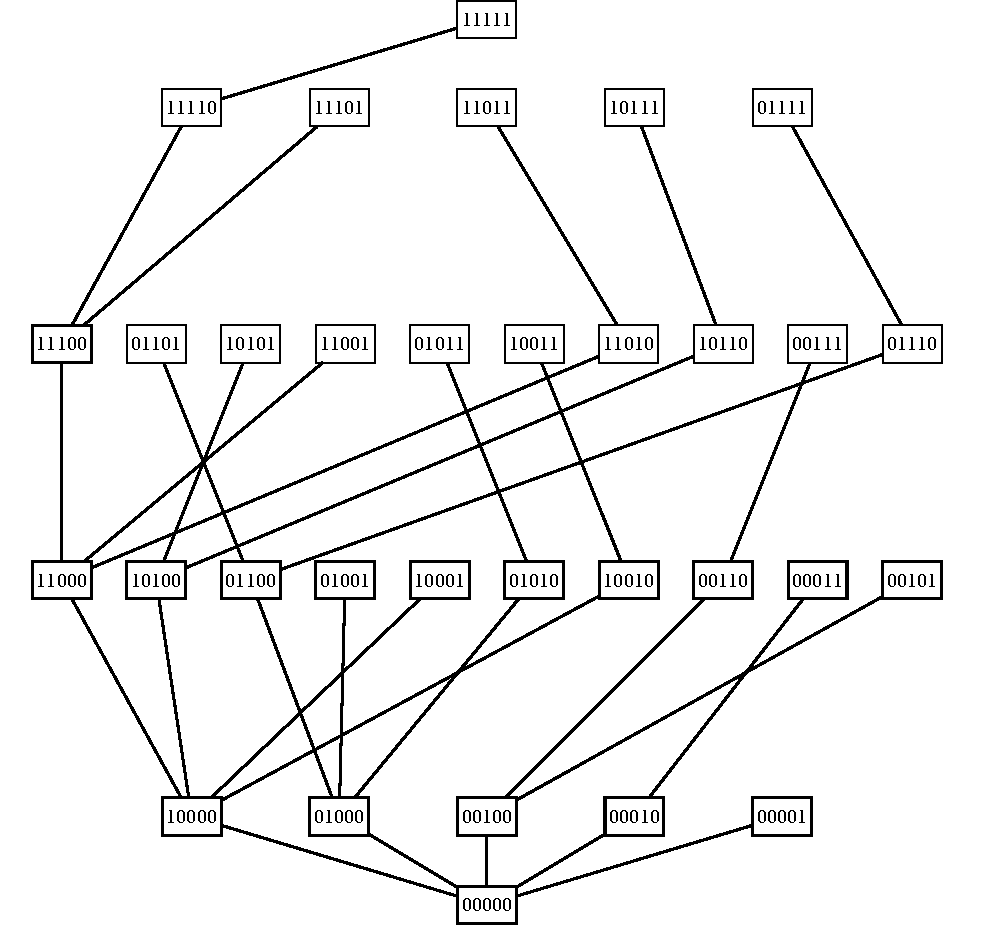
\includegraphics[clip=true]{pfs/pfs/lower_tree.pdf}}
     \label{fig:pfs:lower} }
    & 
    \subfigure[] {\scalebox{.4}{
    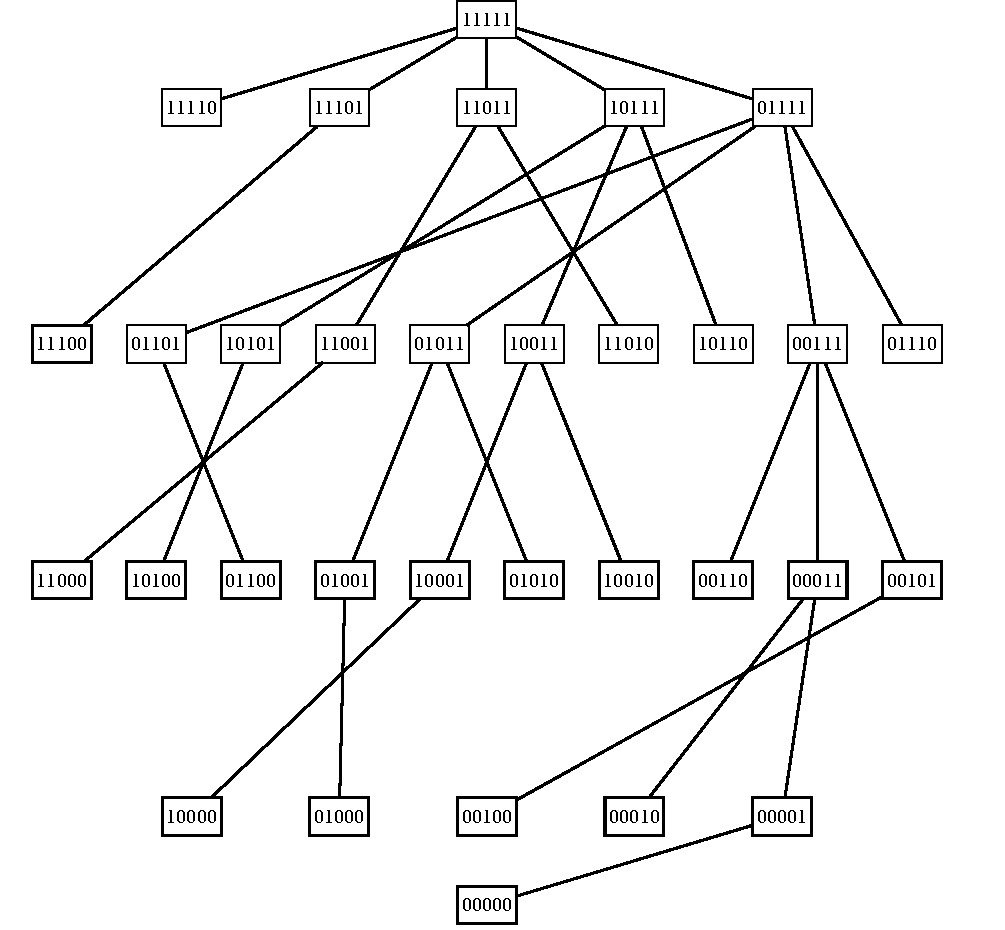
\includegraphics[clip=true]{pfs/pfs/upper_tree.pdf}}
    \label{fig:pfs:upper} }
  \end{tabular}
    \caption{Exemplo de árvores do espaço de busca gerado pelo 
    algoritmo \algname{PFS}. A figura ~\ref{fig:pfs:lower} mostra a 
    árvore gerada por aplicações recursivas do lema 
    ~\ref{lemma:lower_forest} enquanto a figura ~\ref{fig:pfs:upper} 
    mostra a árvore gerada por aplicações recursivas do lema 
    ~\ref{lemma:upper_forest}.}
  \label{fig:pfs:pfs_trees}
\end{figure}



No algoritmo \algname{UBB} o controle do espaço de busca pode ser 
facilmente implementado, pois este começa completo e para cada poda
que ocorre basta não ramificar a sub-árvore em que a condição de poda
for verdadeira, eliminando o intervalo $[Y, X \cup Y]$ do espaço de
busca. No \algname{PFS}, uma estratégia equivalente é capaz apenas de 
restringir nós da estrutura de dados que foi utilizada para o 
percorrimento de cadeias, ou seja, uma poda neste algoritmo implica
na atualização das duas estruturas de dados que controlam o espaço de 
busca. Então, quando removemos um intervalo de uma árvore, precisamos 
remover este mesmo intervalo da árvore dual; como resultado, a árvore 
dual se torna uma {\bf floresta}. Portanto, o \algname{PFS} usa duas
florestas para gerir o espaço de busca, uma com caminhos de conjuntos 
menores para maiores, $\forest_A$ e outra dual, $\forest_B$. Um exemplo
de atualização de floresta dual após uma poda na floresta primal é 
apresentado na figura~\ref{fig:pfs:forest_prune}.

\begin{figure}[!ht]
  \centering 
  \begin{tabular}{c c}
    \subfigure[] {\scalebox{0.4}{
     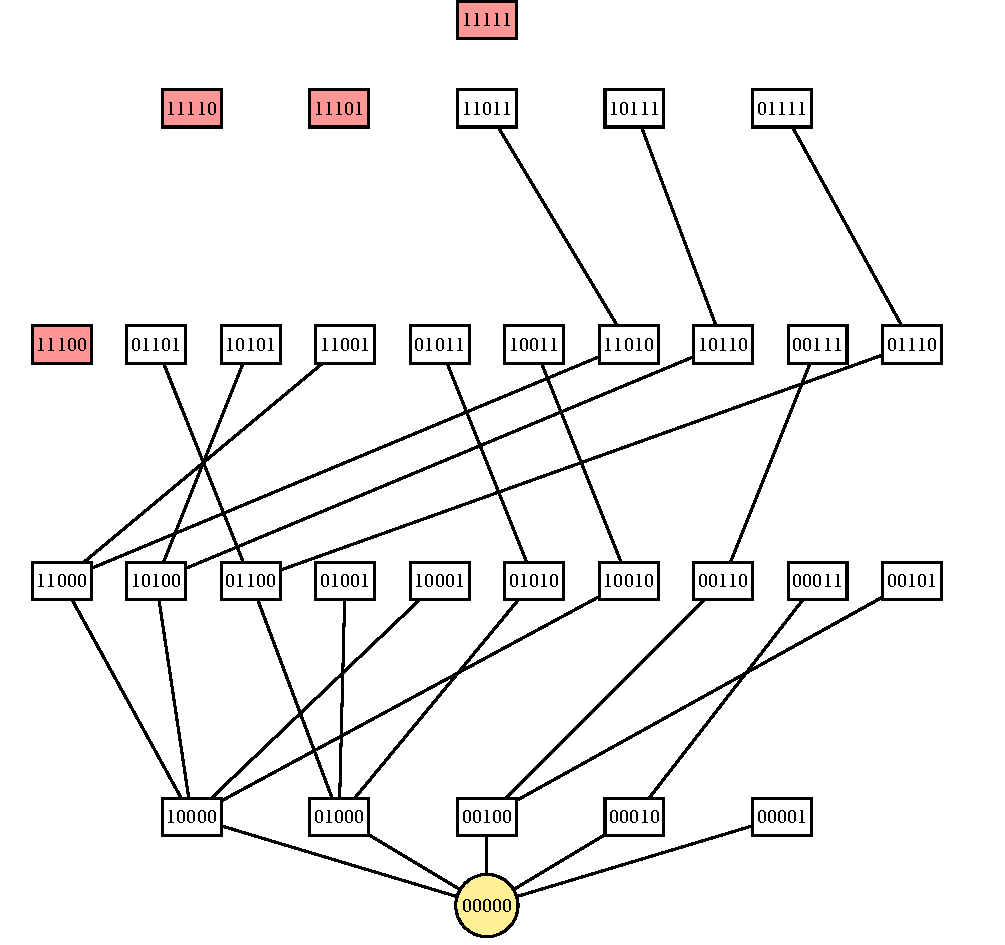
\includegraphics[clip=true]{pfs/pfs/forest/lower_tree.pdf}}
     \label{fig:pfs:forest_pruneA} }
    & 
    \subfigure[] {\scalebox{.4}{
    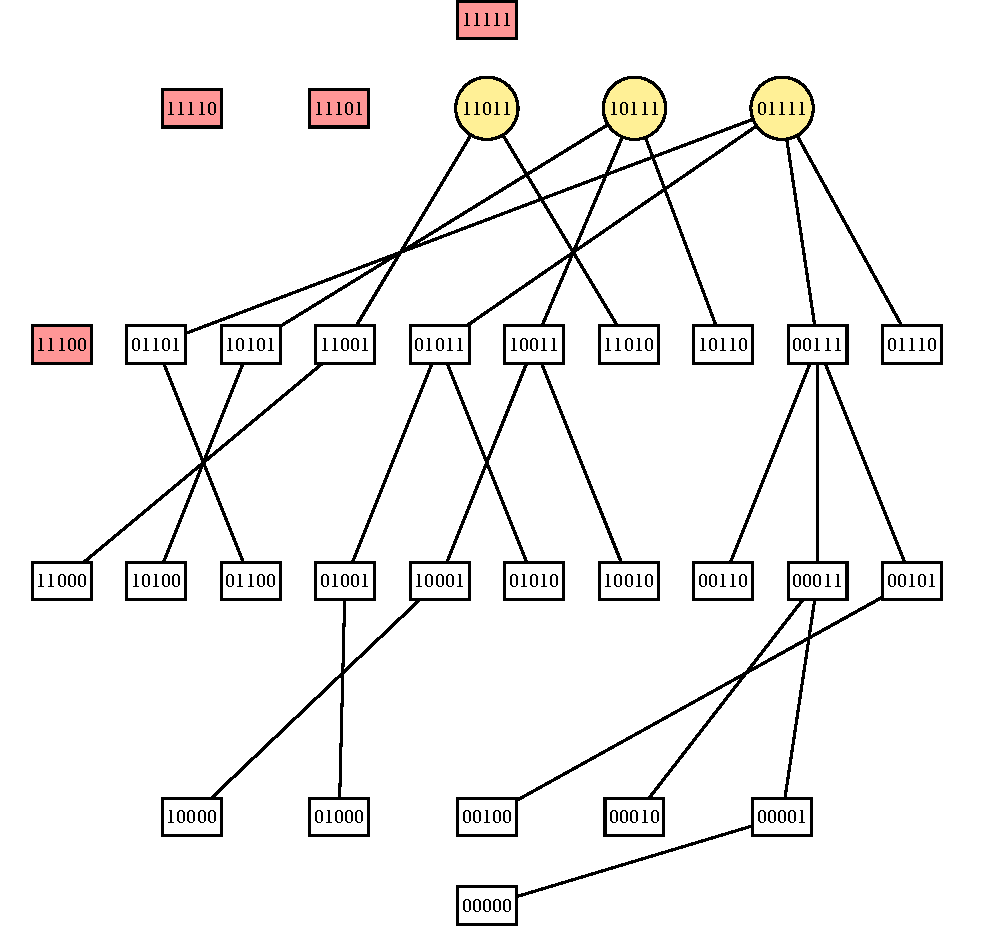
\includegraphics[clip=true]{pfs/pfs/forest/upper_tree.pdf}}
    \label{fig:pfs:forest_pruneB} }
  \end{tabular}
    \caption{Exemplo de atualização de árvore após remoção de intervalo.
    Os nós em vermelho são removidos do espaço de busca enquanto os nós
    amarelos são raízes dos grafos. Removemos o intervalo 
    $[11100, 11111]$ da árvore da figura ~\ref{fig:pfs:forest_pruneA} e 
    ao remover este mesmo intervalo da árvore dual, o grafo perde a 
    raiz original $(11111)$ e ganha as três raízes em amarelo.}
    \label{fig:pfs:forest_prune}
\end{figure}

O \algname{PFS} inicia escolhendo arbitrariamente uma direção de 
percorrimento e uma raiz da floresta correspondente a direção escolhida.
O passo seguinte é a ramificação, que similar ao \algname{UBB} percorre 
uma cadeia da árvore escolhida enquanto o custo dos subconjuntos não 
cresce e não chegamos em uma folha da árvore. Ao fim da fase de 
ramificação, suponha que feita na floresta $\forest_A$ ($\forest_B$),
teremos um intervalo $[Y, X \cup Y]$ ($[Y \setminus X, Y]$) que precisa
ser removido da floresta dual. Esta atualização da floresta dual é 
feita de acordo com as seguintes regras.

\begin{mylemma}
\label{lemma:upper_update}
Sejam $T$ e $T'$ duas árvores tais que $T$ é complementar a $T'$. 
Eliminar de $T'$ os vértices contidos no intervalo $[Y, X \cup Y]$ é 
equivalente a remover de $T'$ todos os vértices do caminho $P$ de $T$ 
com extremos $Y$ e $X \cup Y$ e também todos os vértices de $T'$ 
contidos em intervalos $[Y, B]$ tais que $B$ contém propriamente $Y$ e 
$B$ é adjacente inferior a um vértice de $P$.
\end{mylemma}

\begin{mylemma}
\label{lemma:lower_update}
Sejam $T$ e $T'$ duas árvores tais que $T$ é complementar a $T'$. 
Eliminar de $T$ os vértices contidos no intervalo $[Y \setminus X, Y]$ 
é equivalente a eliminar de $T$ todos os vértices do caminho $P$ em $T$
com extremos $Y \setminus X$ e $Y$ e também todos os vértices de $T$
contidos em intervalos $[A, Y]$ tais que $A$ é contido propriamente em
$Y$ e $A$ é adjacente superior a um vértice de $P$.
\end{mylemma}

As demonstrações dos lemas ~\ref{lemma:upper_update} e 
~\ref{lemma:lower_update} estão disponíveis em Reis ~\cite{Rei12}.

O funcionamento do algoritmo deve seguir as seguintes regras:
\begin{enumerate}[a)]
    \item{\it Inicialização das florestas:} as florestas $\forest_A$ e 
        $\forest_B$ são iniciadas com as raízes $\emptyset$ e $S$ 
        respectivamente. \label{pfs:rule:a}
    \item{\it Representação de árvores:} para todo nó do espaço de busca 
        que não foi removido e não é raiz na floresta, a sub-árvore que
        se inicia neste nó está completa no espaço de buscas. Desta 
        forma, para representar a floresta precisamos apenas armazenar
        as raízes da floresta e suas adjacências, pois sabemos que cada
        vértice adjacente é raiz de uma subárvore completa. 
        \label{pfs:rule:b}
    \item{\it Gerenciamento das florestas:} durante a etapa de 
        ramificação, um vértice visitado é podado ou torna-se raiz na 
        floresta. Com isso, temos que todas arestas de um caminho 
        percorrido são removidas da floresta. \label{pfs:rule:c}
    \item{\it Condição de poda (dual):} no percorrimento de uma cadeia,
        se o nó $Y$ da floresta $\forest_A$ ($\forest_B$) tem custo 
        maior que o último nó visitado nesta cadeia, então removemos da
        floresta $\forest_A$ ($\forest_B$) a subárvore que
        começa em $Y$, $[Y, X \cup Y]$ ($[Y \setminus X, Y]$). Se um nó
        $Y$ visitado não tem conjuntos adjacentes no espaço de busca, 
        então $Y$ é removido do espaço de busca.
        \label{pfs:rule:d}
    \item{\it Atualização de floresta:} ao podar o intervalo 
        $[Y, X \cup Y]$ ($[Y \setminus X, Y]$) da floresta $\forest_A$
        ($\forest_B$), devemos remover os mesmos subconjuntos da outra
        floresta de acordo com o lema ~\ref{lemma:upper_update}
        (\ref{lemma:lower_update}). \label{pfs:rule:e}
\end{enumerate}


\subsection{Pseudo-código e detalhes de implementação do \algname{PFS}}
Apresentamos nesta seção um pseudo-código para o algoritmo e ao mesmo
tempo comentamos como algumas destas soluções foram implementadas em \toolname{C++} no arcabouço \toolname{featsel}.

\subsubsection{Definição de árvores de busca}
Os algoritmos que descrevemos neste capítulo dependem da aplicação 
recursiva dos lemas ~\ref{lemma:lower_forest} e 
~\ref{lemma:upper_forest}, e para cada ordem de características $x_i$
escolhida na aplicação do lema obtemos uma árvore diferente para 
representar o espaço de busca (veja figura ~\ref{fig:pfs:tree_def}). A 
implementação de Reis possui uma enumeração sobre as características 
que nos permite fixar os resultados da aplicação recursiva destes lemas 
e também facilita o controle das árvores da floresta. Supomos então
que o conjunto de características $S$ é uma lista ordenada 
$\langle s_1, s_2, \dots, s_n \rangle$ e que é possível obter o índice 
de um elemento. Assim, sempre que fazemos a decomposição do espaço em 
uma árvore (com ambos lemas) escolhemos as variáveis do conjunto $X$ em
ordem crescente de índice.

\begin{figure}[!ht]
  \centering 
  \begin{tabular}{c c c}
    \subfigure[] {\scalebox{0.7}{
     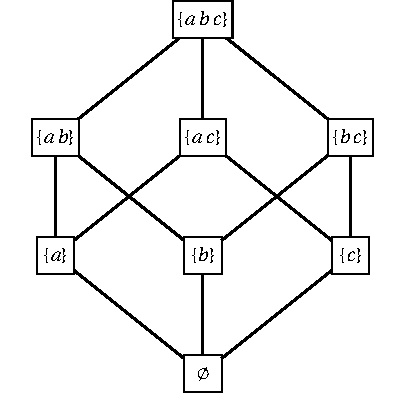
\includegraphics[clip=true]{pfs/feature_enum/original_lattice.pdf}}
     \label{fig:pfs:tree_def:A}}
    & 
    \subfigure[] {\scalebox{.7}{
     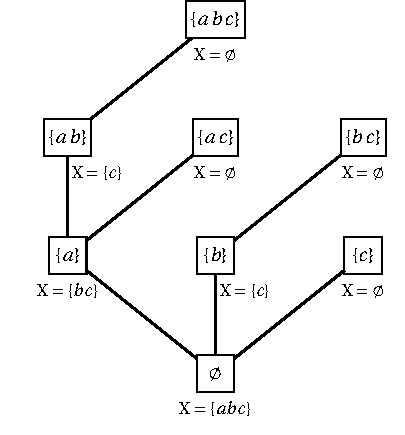
\includegraphics[clip=true]{pfs/feature_enum/treeA.pdf}}
    \label{fig:pfs:tree_def:B}}
    & 
    \subfigure[] {\scalebox{.7}{
     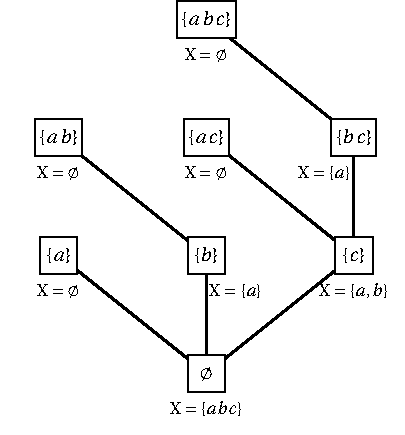
\includegraphics[clip=true]{pfs/feature_enum/treeB.pdf}}
    \label{fig:pfs:tree_def:C}}
  \end{tabular}
    \caption{Exemplos de aplicações recursivas do lema 
    ~\ref{lemma:lower_forest} no reticulado Booleano da figura 
    ~\ref{fig:pfs:tree_def:A}. O conjunto $X$ indica para cada 
    subconjunto $Y$ qual é o conjunto de nós de sua sub-árvore: 
    exatamente os nós do intervalo $[Y, X \cup Y]$. Na figura 
    ~\ref{fig:pfs:tree_def:B} a decomposição elimina de $X$ os elementos
    na ordem $\langle a, b, c \rangle$ em todos os níveis de aplicação 
    do lema, enquanto na figura ~\ref{fig:pfs:tree_def:C} a ordem é 
    $\langle c, b, a \rangle$.}
    \label{fig:pfs:tree_def}
\end{figure}

\subsubsection{Estrutura de dados}
Vamos definir a estrutura de dados utilizada originalmente para representar
nós das florestas. Um nó $\pfsnode{N}$ é composto por quatro campos:
\begin{itemize}
    \item{\varname{vertex}:} armazena o conjunto de características que 
        o nó representa. 
    \item{\varname{adjacent}:} armazena um conjunto de características
        que determina a adjacência do nó. Um nó $\pfsnode{N}$ é 
        adjacente aos conjuntos de características 
        $\{\pfsnode{N}[\varname{vertex}] \cup \{x_i\} : x_i \in \pfsnode{N}[\varname{adjacent}]\}$.
    \item{\varname{leftmost}}: um inteiro que define, pelo esquema de
        numeração, o conjunto de características $X$ da decomposição
        em árvore do espaço de busca. Isto é, se
        $Y = \pfsnode{N}[\varname{vertex}]$ então o conjunto de nós da 
        sub-árvore com raiz $Y$ deve ser igual ao intervalo 
        $[Y, X \cup Y]$, se $\pfsnode{N}$ é da floresta $\forest_A$, ou
        igual ao intervalo $[Y \setminus X, Y]$ se $\pfsnode{N}$ é da 
        floresta $\forest_B$. Lembrando que assumimos uma ordem no 
        conjunto de características ($\langle s_1, s_2, \dots, 
        s_n\rangle$), $X$ é definido como 
            $X = \bigcup_{i = \pfsnode{N}[\varname{leftmost}]}^{n} s_i$.
    \item{$\varname{cost}$:} um número em ponto flutuante que armazena
        o custo de $\pfsnode{N}[\varname{vertex}]$.
\end{itemize}

Como descrevemos na seção anterior, uma das regras do algoritmo garante
que para representar as florestas precisamos apenas armazenar as raízes
das florestas e suas listas de adjacências. Desta maneira, as duas 
florestas $\forest_A$ e $\forest_B$ são representadas por conjuntos de
nós. Estes nós são armazenados na estrutura de \toolname{map} da 
linguagem \langname{C++}. 

\subsubsection{Pseudo-código}
Vamos agora apresentar um pseudo-código do \algname{PFS} em uma 
abordagem ``top down", ou seja, começando pelo algoritmo principal (Algoritmo~\ref{pfs:code:pfs:A}) e descrevendo funções conforme as mesmas são chamadas em um dado pseudo-código.

\begin{algorithm}[]
\textsc{Poset-Forest-Search} $(S, c)$
\begin{algorithmic}[1]
    \State $\mathcal{M} \gets \emptyset$
    \State $\pfsnode{T}[\varname{vertex}] \gets \emptyset$
    \State $\pfsnode{T'}[\varname{vertex}] \gets S$
    \State $\pfsnode{T}[\varname{cost}] \gets \pfsnode{T'}[\varname{cost}] \gets \infty$
    \State $\pfsnode{T}[\varname{adjacent}] \gets \pfsnode{T'}[\varname{adjacent}] \gets S$
    \State $\pfsnode{T}[\varname{leftmost}] \gets \pfsnode{T'}[\varname{leftmost}] \gets 1$
    \State $\forest_A \gets \{\pfsnode{T}\}$
    \State $\forest_B \gets \{\pfsnode{T'}\}$
    \While{$\forest_A \ne \emptyset$} \Comment{equivalent to $\forest_B \ne \emptyset$}
        \State $direction \gets \mathsc{Choose-Direction}$
        \If{$direction$}
            \State $\langle \mathcal{N}, \forest_A, \pfsnode{N} \rangle \gets \mathsc{Lower-Forest-Branch} (\forest_A, \forest_B, c)$
            \State $\forest_B \gets \mathsc{Upper-Forest-Prunning} (\forest_B, \pfsnode{N})$
        \Else
            \State $\langle \mathcal{N}, \forest_A, \pfsnode{N} \rangle \gets \mathsc{Upper-Forest-Branch} (\forest_A, \forest_B, c)$
            \State $\forest_A \gets \mathsc{Lower-Forest-Prunning} (\forest_A, \pfsnode{N})$
        \EndIf
        \State $\mathcal{M} \gets \mathcal{M} \cup \mathcal{N}$
    \EndWhile
    \Return $\{M \in \mathcal{M} : c(M) \text{ is minimum}\}$
\end{algorithmic}
\vspace{1em}
\caption{Pseudo-código da rotina principal do algoritmo \algname{PFS}.}
\label{pfs:code:pfs:A}
\end{algorithm}

Uma iteração qualquer do \algname{PFS} começa com a inicialização das 
florestas do espaço de busca. A floresta $\forest_A$, que permite 
percorrimentos de baixo para cima no reticulado, é inicializada com 
a raiz $\emptyset$, enquanto que a floresta $\forest_B$, de percorrimentos
de cima para baixo, é inicializada com a raiz $S$. Assim que 
inicializadas as florestas, repetimos as etapas de escolha de direção
de percorrimento, ramificação e poda das florestas até que ambas 
estejam vazias. Note que não importa qual floresta devemos verificar
para terminar as iterações do algoritmo, já que ambas representam o 
mesmo espaço de busca, ou seja, quando uma floresta é vazia a outra 
também é.


A etapa de ramificação da floresta $\forest_A$ é feita pela função 
\textsc{Lower-Forest-Branch} (Algoritmo~\ref{pfs:code:pfs:B}) e consiste no percorrimento, a partir de uma 
raiz $Y$, de uma cadeia de sua sub-árvore. Nesta etapa, para manter 
válida a regra~\ref{pfs:rule:c} devemos remover todas as arestas do 
caminho percorrido e transformar todos os nós visitados e não podados em 
raízes da floresta. O percorrimento termina ao atingir um nó 
$\pfsnode{N}$ que é folha ou que possui custo maior do que seu 
precedente no caminho percorrido; então o intervalo 
$[\pfsnode{N}[\varname{vertex}], \pfsnode{N}[\varname{vertex}] \cup \pfsnode{N}[\varname{adjacent}]]$
deve ser removido da floresta $\forest_A$. Esta função retorna o nó 
$\pfsnode{N}$, a floresta $\forest_A$ atualizada, e o conjunto 
$\mathcal{M}$ de subconjuntos percorridos que são candidatos a mínimo.

\begin{algorithm}[ht]
\textsc{Lower-Forest-Branch} $(\forest_A, \forest_B, c)$
\begin{algorithmic}[1]
    \State $\mathcal{M} \gets \emptyset$
    \State remova um nó $\pfsnode{R}$ de $\forest_A$
    \State $\pfsnode{R}[\varname{cost}] \gets \mathsc{Calc-Node-Cost}(\forest_B, \pfsnode{R})$
    \State $\pfsnode{M} \gets \pfsnode{N} \gets \pfsnode{R}$
    \While{$\pfsnode{N}[\varname{cost}] \leq \pfsnode{M}[\varname{cost}]$ e $\pfsnode{N}[\varname{adjacent}] \ne \emptyset$}
        \State $\pfsnode{M} \gets \pfsnode{N}$
        \State remova um elemento de $s_i$ de $\pfsnode{M}[\varname{adjacent}]$
        \State $\forest_A \gets \forest_A \cup \{\pfsnode{M}\}$
        \State crie o nó $\pfsnode{N}$
        \State $\pfsnode{N}[\varname{vertex}] \gets \pfsnode{M}[\varname{vertex}] \cup \{s_i\}$
        \State $\pfsnode{N}[\varname{leftmost}] \gets i$
        \State $\pfsnode{N}[\varname{adjacent}] \gets \bigcup_{i=\pfsnode{N}[\varname{leftmost}]}^{n} s_i$
        \State $\pfsnode{N}[\varname{cost}] \gets \mathsc{Calc-Node-Cost} (\forest_B, \pfsnode{N})$
        \State $\mathcal{M} \gets \mathcal{M} \cup \{\pfsnode{N}\}$
    \EndWhile
    \Return $\langle \mathcal{M}, \forest_A, \pfsnode{N}\rangle$
\end{algorithmic}
\caption{Pseudo-código da função que faz o percorrimento da floresta $\forest_A$.}
\label{pfs:code:pfs:B}
\end{algorithm}

Durante a execução do \algname{PFS}, o custo de um subconjunto é calculado uma única vez; o recálculo é evitado com a função \algname{Calc-Node-Cost} (Algoritmo~\ref{alg:Calc-Node-Cost}).

\begin{algorithm}[H]
\textsc{Calc-Node-Cost} $(\forest, \pfsnode{N})$
\begin{algorithmic}[1]
\If{$\pfsnode{N}[\varname{cost}] = \infty$ e existe $\pfsnode{M} \in \forest$ tal que $\pfsnode{M}[\varname{vertex}] = \pfsnode{N}[\varname{vertex}]$ e $\pfsnode{M}[\varname{cost}] \ne \infty$}
    \Return $\pfsnode{M}[\varname{cost}]$
\Else
    \Return $c(\pfsnode{R}[\varname{vertex}])$
\EndIf
\end{algorithmic}
\caption{Pseudo-código da função \algname{Calc-Node-Cost}.}
\label{alg:Calc-Node-Cost}
\end{algorithm}

A ramificação dual, da floresta $\forest_B$ é feita pela função 
\textsc{Upper-Forest-Branch} e é similar a função 
\textsc{Lower-Forest-Branch} ao percorrer uma cadeia da floresta de 
conjuntos maiores para conjuntos menores. A ramificação termina ao 
encontrar um nó $\pfsnode{N}$ que é folha da floresta ou tem custo maior
que seu precedente no caminho; então o intervalo 
$[\pfsnode{N}[\varname{vertex}] \setminus \pfsnode{N}[\varname{adjacent}], \pfsnode{N}[\varname{vertex}]]$
deve ser removido da floresta $\forest_B$ e todos os nós visitados, 
menos $\pfsnode{N}$ tornam-se raízes. Esta função retorna o nó
$\pfsnode{N}$, a floresta $\forest_B$ atualizada e o conjunto 
$\mathcal{M}$ de subconjuntos percorridos que são candidatos a mínimo.

A atualização da floresta $\forest_B$ após o percorrimento e poda da
floresta $\forest_A$ é feito pela função \textsc{Upper-Forest-Prunning} (Algoritmo~\ref{pfs:code:pfs:C}).
Esta função recebe um nó $\pfsnode{N}$ e deve remover os nós de 
$\forest_B$ de acordo com a regra ~\ref{pfs:rule:e}. Para fazer isto, 
percorremos o caminho $P$ que liga os nós de subconjuntos 
$\pfsnode{N}[\varname{vertex}]$ e $\pfsnode{N}[\varname{vertex}] \cup 
\pfsnode{N}[\varname{adjacent}]$ na floresta $\forest_B$, removendo cada
um dos nós deste caminho (se existirem, o que é verificado pela função descrita no algoritmo~\ref{alg:Get-Node}) e chamando a função 
\textsc{Search-Lower-Children} (Algoritmo~\ref{pfs:code:pfs:D}) para verificar se os filhos destes nós
devem ser podados ou não. Ao fim do caminho chamamos a função 
\textsc{Search-Upper-Root} para achar, na floresta $\forest_B$, a raiz
que alcança este caminho e atualizar a sua adjacência  para garantir que 
uma ramificação não vai re-inserir os nós removidos. 
Esta função devolve a floresta $\forest_B$ atualizada.

\begin{algorithm}[H]
    \textsc{Uppper-Forest-Prunning} ($\forest_A, \forest_B, \pfsnode{N}$)
    \begin{algorithmic}[1]
        \State $M \gets \pfsnode{N}[\varname{vertex}]$
        \While{$\pfsnode{N}[\varname{adjacent}] \ne \emptyset$}
            \State $\pfsnode{M} \gets \mathsc{Get-Node} (\forest_B, M)$
            \If{$\pfsnode{M} \ne NIL$}
                \State remova $\pfsnode{M}$ de $\forest_B$
            \EndIf
            \State $\forest_B \gets \mathsc{Search-Lower-Children} (\forest_B, \pfsnode{M}, M, \pfsnode{N}[\varname{vertex}])$
            \State remova o elemento $s_i$ de $\pfsnode{N}[\varname{adjacent}]$ com maior $i$
            \State $M \gets M \cup \{s_i\}$
        \EndWhile
        \State $\pfsnode{M} \gets \mathsc{Get-Node} (\forest_B, M)$
        \If{$\pfsnode{M} = NIL$}
            \State $\mathsc{Search-Upper-Root} (\forest_B, M)$
        \Else
            \State remova $\pfsnode{M}$ de $\forest_B$
        \EndIf
        \State $\forest_B \gets \mathsc{Search-Lower-Children} (\forest_B, \pfsnode{M}, M, \pfsnode{N}[\varname{vertex}])$
        \Return $\forest_B$
    \end{algorithmic}
    \caption{Pseudo-código da função que faz a atualização da floresta $\forest_B$ depois de um 
    percorrimento em $\forest_A$.}
    \label{pfs:code:pfs:C}
\end{algorithm}

\begin{algorithm}[H]
    \textsc{Get-Node} ($\forest, N$)
    \begin{algorithmic}[1]
        \If{existe $\pfsnode{N} \in \forest$ tal que $\pfsnode{N}[\varname{vertex}] = N$}
            \Return $\pfsnode{N}$
        \Else
            \Return $NIL$
        \EndIf
    \end{algorithmic}
\caption{Pseudo-código da função \algname{Get-Node}.}
\label{alg:Get-Node}
\end{algorithm}

\begin{algorithm}[H]
\textsc{Search-Lower-Children} $(\forest_B, \pfsnode{M}, M, Y)$
\begin{algorithmic}[1]
    \State $i \gets n$
    \While{$i \geq 1$ e $s_i \in M$}
        \State $B \gets M \setminus \{s_i\}$
        \If{$B \supseteq Y$}
            \State $\pfsnode{B} \gets \mathsc{Get-Node} (\forest_B, M)$
            \If{$\pfsnode{B} \ne NIL$}
                \State remova $\pfsnode{B}$ de $\forest_B$
            \EndIf
        \Else
            \State crie o nó $\pfsnode{B}$
            \State $\pfsnode{B}[\varname{vertex}] \gets B$
            \State $\pfsnode{B}[\varname{leftmost}] \gets i + 1$
            \State $\pfsnode{B}[\varname{adjacent}] \gets \bigcup_{i=\pfsnode{B}[\varname{leftmost}]}^{n} s_i$
            \State $\pfsnode{B}[\varname{cost}] \gets \infty$
            \State $\forest_B \gets \forest_B \cup \{\pfsnode{B}\}$ 
        \EndIf
        \State $i \gets i - 1$
        \Return $\forest_B$
    \EndWhile
\end{algorithmic}
\caption{Pseudo-código da função \algname{Search-Lower-Children}.}
\label{pfs:code:pfs:D}
\end{algorithm}

A atualização dual, da floresta $\forest_A$, após o percorrimento e 
poda da floresta $\forest_B$ é feito pela função 
\textsc{Lower-Forest-Pruning} e seu funcionamento é parecido com o de
\textsc{Upper-Forest-Pruning}. O caminho $P$ de $\forest_A$ que deve 
ser removido tem as pontas 
$\pfsnode{N}[\varname{vertex}] \setminus \pfsnode{N}[\varname{adjacent}]$
e $\pfsnode{N}[\varname{vertex}]$, e a função 
\textsc{Search-Upper-Children} é chamada para verificar se os filhos 
destes nós devem ser podados ou não. Ao fim do caminho chamamos a função 
\textsc{Search-Lower-Root} para achar, na floresta $\forest_A$, a raiz
que alcança este caminho e atualizar a sua adjacência para garantir que 
uma ramificação não vai re-inserir os nós removidos. Esta função devolve 
a floresta $\forest_A$ atualizada.

A função \textsc{Search-Lower-Children} é chamada para cada nó $M$ do 
caminho $P$, como descrito no lema ~\ref{lemma:upper_update}. Esta 
função verifica para todos os filhos $B$ de $M$ se $B$ contém 
propriamente o conjunto $\pfsnode{N}[\varname{vertex}]$; se contém, o 
nó de subconjunto $B$ deve ser removido da floresta, caso 
contrário, um nó que representa este conjunto deve ser tornar raiz da 
floresta, pois o pai de $B$ está sendo removido da floresta e isto 
significa que não haverá raiz que alcance $B$. Esta função
devolve a floresta $\forest_B$ atualizada. \textsc{Search-Upper-Children} é a função dual de 
\textsc{Search-Lower-Children} e faz um procedimento similar, para 
cada nó $\pfsnode{M}$ do caminho $P$, como descrito no lema 
~\ref{lemma:lower_update}. Esta função verifica para todos os filhos $A$
de $M$ se $A$ é contido propriamente pelo conjunto 
$\pfsnode{N}[\varname{vertex}]$; se é, o nó de subconjunto $A$ deve ser 
removido da floresta, caso contrário, o um nó que representa o conjunto 
$A$ deve se tornar raiz da floresta. Esta função devolve a floresta 
$\forest_A$ atualizada.


Por fim, a função \textsc{Search-Upper-Root} (Algoritmo~\ref{alg:Search-Upper-Root}) recebe um subconjunto $M$ e a 
floresta $\forest_B$. O objetivo desta função é remover arestas da 
floresta que podem levar ao conjunto $M$. Para isto, a função deve 
percorrer um caminho de $M$ até uma raiz da floresta (de conjuntos 
menores para maiores), e esta raiz deve ter sua lista de adjacência 
atualizada, removendo a aresta que a comunica com $M$. Para garantir que 
removemos todas as arestas, devemos criar raízes para todos nós deste 
caminho mas sem a adjacência que os comunica com $M$. O funcionamento de 
\textsc{Search-Lower-Root} é similar, mas deve ocorrer em outra direção
(de conjuntos maiores para menores).

\begin{algorithm}[H]
\textsc{Search-Upper-Root} $(\forest_B, M)$
\begin{algorithmic}[1]
    \State $i \gets n$
    \While{$i \geq 1$ e $s_i \in M$}
        \State $i \gets i - 1$
    \EndWhile
    \While{$i \geq 1$}
        \State $m \gets s_i$
        \State $M \gets M \cup \{m\}$
        \State $\pfsnode{M} \gets \mathsc{Get-Node} (\forest_B, M)$
        \If{$\pfsnode{M} \ne NIL$}
            \State $\pfsnode{M}[\varname{adjacent}] \gets \pfsnode{M}[\varname{adjacent}] \setminus \{m\} $
            \State $i \gets 0$
        \Else
            \State crie o nó $\pfsnode{M}$
            \While{$i \geq 1$ e $s_i \in M$}
                \State $i \gets i - 1$
            \EndWhile
            \State $\pfsnode{M}[\varname{leftmost}] \gets i + 1$
            \State $\pfsnode{M}[\varname{adjacent}] \gets \cup_{j = \pfsnode{M}[\varname{leftmost}]}^{n} \{s_j\} \setminus \{m\} $
            \State $\pfsnode{M}[\varname{cost}] \gets \infty$
            \State adicione $\pfsnode{M}$ em $\forest_B$
        \EndIf
        \Return $\forest_B$
    \EndWhile
\end{algorithmic}
\caption{Pseudo-código da função~\algname{Search-Upper-Root}.}
\label{alg:Search-Upper-Root}
\end{algorithm}

\section{Melhoramentos na escolha de raiz}
% - começar falando sobre o problema... 
%   a escolha era feita de maneira arbitrária. Estrutura de map guardava
%   as raízes e escolhia-se o primeiro elemento do map, que de acordo com
%   será o menor elemento lexicograficamente ou o maior 
% - por que mudar isso pode melhorar? Porque o critério é arbitrário
% - aleatória: talvez traga melhoras se a abordagem anterior escolhesse 
%   raízes ruins
% - "leftmost": estamos priorizando percorrer as maiores árvores, em 
%   tese
Na implementação original do \algname{PFS} foi utilizada a estrutura de \toolname{map} para armazenar as raízes das 
florestas do espaço de busca. Como chave das raízes, utiliza-se a 
\toolname{string} que representa o vetor característico da raiz. A 
estrutura de \toolname{map} em \langname{C++}, geralmente implementada
com árvores binárias de busca, mantém os elementos ordenados pelo valor
de sua chave, portanto as raízes são armazenadas de maneira ordenada
lexicograficamente.

A estratégia adotada na implementação original para a escolha de uma raiz da floresta 
consiste em escolher de maneira equiprovável o primeiro ou o último 
elemento do \toolname{map} de raízes. Esta estratégia é aleatória, porém viesada, uma vez que escolhe apenas os primeiros ou últimos elementos de uma ordenação. Como esta estratégia de ordenação é arbitrária, não existindo fundamentação teórica que a justifique, acreditamos que novas 
estratégias de escolhas de raízes podem trazer melhores resultados ao algoritmo \algname{PFS}.

\subsection{Escolha equiprovável}
A primeira estratégia que testamos foi uma escolha também aleatória, mas
com uma distribuição de probabilidade de escolhas igual para cada raiz
da floresta. Como a estratégia da implementação original de Reis é viesada, julgamos necessário
investigar se este viés não leva o algoritmo a fazer ramificações ou 
podas ruins, que comprometessem o tempo de execução do algoritmo. Se
o tempo de execução com a nova estratégia é menor, então confirmamos
esta hipótese.

Para implementar esta nova escolha, utilizamos a mesma estrutura de 
dados utilizada por Reis com uma pequena modificação no código. Seja
$\forest$ a floresta de percorrimento escolhida e suponha que existe
uma ordenação das raízes dessa floresta, 
$\langle r_1, r_2, ..., r_{|\forest|} \rangle$, então sorteamos um 
número $i$ entre $1$ e $|\forest|$ e escolhemos a raiz $r_{i}$ para o
percorrimento.


\subsection{Escolha de maior árvore}
A segunda estratégia que testamos para escolha de raízes é 
determinística e se baseia em escolher a raiz que tem maior 
sub-árvore completa. Acreditamos que este critério pode acelerar o
algoritmo porque árvores maiores podem fazer podas maiores e, desta 
maneira, é possível que o algoritmo precise visitar menos nós do 
reticulado e portanto fazer menos operações, incluindo menos cálculos
da função custo.

A sub-árvore completa que tem como raiz o nó $\pfsnode{N}$ é composta 
pelos nós dos conjuntos do intervalo 
$[\pfsnode{N}[\varname{vertex}], \pfsnode{N}[\varname{vertex}] \cup \pfsnode{N}[\varname{adjacent}]]$ e 
portanto, o tamanho da árvore é dado por
\begin{subequations}
\begin{align*}
|[\pfsnode{N}[\varname{vertex}], \pfsnode{N}[\varname{vertex}] \cup \pfsnode{N}[\varname{adjacent}]]| &= 
|\{\pfsnode{N}[\varname{vertex}] \cup W : W \in \powerset (\pfsnode{N}[\varname{adjacent}])\}| \\
    &= |\powerset(\pfsnode{N}[\varname{adjacent}])| \\
    &= |\powerset(\cup_{i = \pfsnode{N}[\varname{leftmost}]}^{n} s_i)| \\
    &= 2^{n - \pfsnode{N}[\varname{leftmost}]}.
\end{align*}
\end{subequations}
Portanto, basta escolher a raiz com menor valor de $\varname{leftmost}$.
Agora note que, para as raízes da floresta $\forest_A$, o valor de 
$\varname{leftmost}$ é igual ao maior índice de uma característica
presente no conjunto, enquanto na floresta $\forest_B$ é igual ao maior
índice de uma característica não presente no conjunto.

Note que este número considera que a árvore está completa, o que não é
necessariamente verdade para raízes da floresta; um cálculo exato 
deveria considerar também o conjunto $\varname{adjacent}$ da raiz. 
Entretanto, utilizamos esse cálculo como uma aproximação do tamanho da 
floresta por motivos de simplicidade, pois, como explicaremos a seguir,
podemos ordenar as raízes de maneira rápida utilizando este cálculo 
aproximado; fazer esta ordenação com um cálculo que considera as 
adjacências pode não ser simples.

Se ordenamos as raízes de forma lexicográfica da direita
para esquerda (da característica com maior índice para característica
com menor índice). Então, a menor raiz é aquela que possui mais zeros
da direita para esquerda, ou seja, o menor valor para o maior índice
de uma característica presente e consequentemente o menor 
$\varname{leftmost}$ da floresta $\forest_A$. Já a maior raiz é aquela 
que possui mais uns da direita para esquerda, ou seja, o menor valor 
para o maior índice de uma característica não presente e 
consequentemente o maior $\varname{leftmost}$ da floresta $\forest_B$.

Portanto, para implementar esta modificação devemos mudar o tipo de
ordenação feito pelo \toolname{map}, que por padrão é feito 
lexicograficamente da esquerda para direita (ordem alfabética), e 
escolher para floresta $\forest_A$ o primeiro elemento do \toolname{map}
e para a floresta $\forest_B$ o último elemento.


\subsection{Experimentos com instâncias artificiais}
\label{pfs:root_choosing:experiments}
Testamos ambas abordagens em experimentos computacionais. Analisaremos agora o desempenho dos 
algoritmos tanto quanto ao tempo médio de execução quanto a quantidade
média de nós computados.

A tabela \ref{tab:pfsrand_vs_pfs} mostra os resultados dos 
experimentos para os algoritmos \algname{PFS} e sua variante que 
seleciona raízes de maneira aleatória e igualmente distribuída, o que 
chamamos de \algname{PFS\_RAND}. Podemos perceber na tabela que o número
de chamadas de função custo tem média e variância parecidas em ambos 
algoritmos. O tempo médio de execução, por outro lado, é maior para o
algoritmo \algname{PFS\_RAND}. Portanto, podemos concluir que a
esta modificação do \algname{PFS} não trouxe melhorias nos quesitos
que estamos avaliando.

\begin{table}
\centering
\footnotesize
\caption{Comparação entre os algoritmos \algname{PFS} e 
\algname{PFS\_RAND}. O tempo de execução do segundo é maior do que o 
primeiro enquanto a quantidade de chamadas da função custo é parecida
em ambos.} \label{tab:pfsrand_vs_pfs}
 \resizebox{\columnwidth}{!}{%
\begin{tabular}{cc c cc c cc}
\toprule
\multicolumn{2}{c}{Instância} & \phantom{} & \multicolumn{2}{c}{Tempo de execução médio (s)}  & \phantom{} & \multicolumn{2}{c}{Número médio de cálculos de custo}\\
\cline{1-2}\cline{4-5}\cline{7-8}\\
$|S|$ & $2^{|S|}$ && \algname{PFS} & \algname{PFS\_RAND} && \algname{PFS} & \algname{PFS\_RAND} \\
10 &    1024 &&  0.013 $\pm$ 0.003 & 0.014 $\pm$ 0.003 &&   590.8 $\pm$ 198.5 & 599.5 $\pm$ 177.5 \\
11 &    2048 &&  0.019 $\pm$ 0.004 & 0.022 $\pm$ 0.007 &&   1114.8 $\pm$ 331.3 & 1090.1 $\pm$ 350.3 \\
12 &    4096 &&  0.029 $\pm$ 0.008 & 0.036 $\pm$ 0.013 &&   1848.6 $\pm$ 600.8 & 1835.7 $\pm$ 683.0 \\
13 &    8192 &&  0.060 $\pm$ 0.018 & 0.090 $\pm$ 0.039 &&   4314.4 $\pm$ 1496.4 & 4201.1 $\pm$ 1580.7 \\
14 &   16384 &&  0.100 $\pm$ 0.041 & 0.191 $\pm$ 0.110 &&   7323.4 $\pm$ 3318.9 & 7333.8 $\pm$ 3161.0 \\
15 &   32768 &&  0.180 $\pm$ 0.076 & 0.453 $\pm$ 0.311 &&   12958.1 $\pm$ 5654.0 & 12807.5 $\pm$ 5753.7 \\
16 &   65536 &&  0.406 $\pm$ 0.185 & 1.715 $\pm$ 1.400 &&   27573.8 $\pm$ 12459.5 & 27036.9 $\pm$ 12687.5 \\
17 &  131072 &&  0.717 $\pm$ 0.397 & 5.416 $\pm$ 5.266 &&   48176.2 $\pm$ 26938.3 & 47852.1 $\pm$ 26427.6 \\
18 &  262144 &&  1.325 $\pm$ 0.754 & 15.890 $\pm$ 17.726 &&   84417.9 $\pm$ 48587.7 & 84025.0 $\pm$ 48882.4 \\
19 &  524288 &&  2.771 $\pm$ 1.603 & 69.600 $\pm$ 82.342 &&   167659.1 $\pm$ 99686.7 & 164612.1 $\pm$ 102018.3 \\
\bottomrule
\end{tabular}%
 }

\end{table}
 
A tabela \ref{tab:pfsleftmost_vs_pfs} mostra os resultados dos 
experimentos para os algoritmos \algname{PFS} e sua variante que 
seleciona a raiz com maior potencial de poda, o que chamamos de 
\algname{PFS\_LEFTMOST}. A tabela mostra que o último algoritmo 
teve desempenho pior em tempo de execução e fez mais chamadas da 
função de custo, isto é, percorreu mais nós do que o \algname{PFS}.
Assim, concluímos que esta modificação não foi vantajosa ao algoritmo.

\begin{table}
\centering
\footnotesize
\caption{Comparação entre os algoritmos \algname{PFS} e 
\algname{PFS\_LEFTMOST}. O tempo de execução e também o número de 
chamadas da função custo é maior para o \algname{PFS\_LEFTMOST}.} 
\label{tab:pfsleftmost_vs_pfs}
 \resizebox{\columnwidth}{!}{%
\begin{tabular}{cc c cc c cc}
\toprule
\multicolumn{2}{c}{Instância} & \phantom{} & \multicolumn{2}{c}{Tempo de execução médio (s)}  & \phantom{} & \multicolumn{2}{c}{Número médio de cálculos de custo}\\
\cline{1-2}\cline{4-5}\cline{7-8}\\
$|S|$ & $2^{|S|}$ && \algname{PFS} & \algname{PFS\_LEFTMOST} && \algname{PFS} & \algname{PFS\_LEFTMOST} \\
10 &    1024 &&  0.013 $\pm$ 0.002 & 0.023 $\pm$ 0.004 &&  606.1 $\pm$ 133.5 & 665.0 $\pm$ 165.8 \\
11 &    2048 &&  0.020 $\pm$ 0.004 & 0.042 $\pm$ 0.010 &&  1122.1 $\pm$ 351.2 & 1316.6 $\pm$ 382.2 \\
12 &    4096 &&  0.032 $\pm$ 0.008 & 0.078 $\pm$ 0.024 &&  2183.7 $\pm$ 733.2 & 2515.8 $\pm$ 871.3 \\
13 &    8192 &&  0.054 $\pm$ 0.017 & 0.160 $\pm$ 0.061 &&  3887.7 $\pm$ 1389.9 & 4716.8 $\pm$ 1777.8 \\
14 &   16384 &&  0.107 $\pm$ 0.034 & 0.345 $\pm$ 0.133 &&  7851.2 $\pm$ 2793.0 & 9506.8 $\pm$ 3673.9 \\
15 &   32768 &&  0.196 $\pm$ 0.085 & 0.672 $\pm$ 0.274 &&  13780.3 $\pm$ 6049.9 & 17071.6 $\pm$ 7005.1 \\
16 &   65536 &&  0.348 $\pm$ 0.189 & 1.271 $\pm$ 0.661 &&  24106.5 $\pm$ 13159.9 & 30055.6 $\pm$ 15363.6 \\
17 &  131072 &&  0.785 $\pm$ 0.361 & 3.137 $\pm$ 1.476 &&  52369.0 $\pm$ 24751.2 & 67585.6 $\pm$ 30978.4 \\
18 &  262144 &&  1.445 $\pm$ 0.657 & 6.146 $\pm$ 3.032 &&  92095.9 $\pm$ 42566.6 & 120635.7 $\pm$ 58039.0 \\
19 &  524288 &&  3.298 $\pm$ 1.883 & 13.881 $\pm$ 7.595 &&  199151.0 $\pm$ 112167.8 & 256078.6 $\pm$ 135958.4 \\
20 & 1048576 &&  6.141 $\pm$ 3.728 & 28.733 $\pm$ 18.120 &&  356259.2 $\pm$ 218253.1 & 465255.8 $\pm$ 276843.3 \\
21 & 2097152 &&  10.817 $\pm$ 7.714 & 52.374 $\pm$ 38.565 &&  608984.4 $\pm$ 432151.7 & 801620.2 $\pm$ 561000.7 \\
\bottomrule 
\end{tabular}%
 }
\end{table}

\subsection{Comentários sobre experimentos}
Os experimentos mostraram que a modificação \algname{PFS\_RAND} teve um
número parecido de chamadas da função custo. Pelo fato destes números
serem parecidos, acreditamos que o percorrimento do reticulado também 
seja parecido, o que implica que semanticamente esta modificação é 
equivalente ao algoritmo original. Entretanto, observamos que o
\algname{PFS\_RAND} teve tempo de execução médio maior. Na busca por
entender como o algoritmo pode ter ficado mais caro computacionalmente
se sua dinâmica é essencialmente a mesma, investigamos a estrutura de
\algname{map} do \langname{C++} e descobrimos que a forma com que implementamos 
a escolha aleatória de um elemento desta estrutura, avançando um 
iterador por uma quantidade aleatória de passos, adiciona tempo de 
complexidade linear (sobre o número de raízes) ao algoritmo, 
justificando o aumento de tempo de execução.

A outra modificação, \algname{PFS\_LEFTMOST}, não tem adições de 
complexidade computacional na escolha de raízes, visto que ela é feita
da mesma forma no algoritmo original, apenas com diferente regra de 
ordenação. Esta modificação teve um número maior de cálculos da função
de custo, o que significa que mais elementos do reticulado foram
percorridos (menos foram podados) e também explica o maior tempo de 
execução. Podemos concluir que esta modificação não é semanticamente 
equivalente ao \algname{PFS} porque implica em um percorrimento 
diferente do espaço de busca, evidenciado por mais cálculos da função 
custo.


\section{Melhoramentos no controle de raízes}
% - quando o número de raízes é muito grande map é uma estrutura mais 
%   cara para consultas e inserções, enquanto nas ROBDDs essa operação é 
%   mais barata(?)
% - o número de raízes na floresta pode crescer muito: no pior caso, 
%   todos os nós do reticulado podem ser raízes!
%     - explicar ROBDDs
% - uso de ROBDD
%   com raíz aleatória e com raíz leftmost
A quantidade de raízes em uma floresta pode ser muito grande no decorrer 
do algoritmo \algname{PFS}. Um pior caso, exagerado, é considerar que 
os percorrimentos foram feitos sempre em uma das florestas e que a 
função de custo é monótona tal que não houveram podas por conta de 
aumento de custo; então, esta floresta poderá ter até $2^n - n + 1$ 
raízes. Desta forma, a estrutura de dados utilizada para gerenciar a 
floresta deve ser eficiente e capaz de armazenar muitas entradas.
A estrurura \toolname{map} do 
\langname{C++} é implementada através de uma árvore rubro-negra, uma árvore de busca binária que é balanceada mas não ordenada. Por isso, acreditamos que outras estruturas devem ser consideradas para gerenciar as raízes das 
florestas do \algname{PFS}. Desta maneira, podemos encontrar novas 
estruturas mais eficientes para o problema.

Introduzimos então o uso de diagramas de decisão binária ordenados 
(Ordered Binary Decision Diagram (OBDD)). Esta estrutura representa uma
função Booleana $f : \{0, 1\}^k \to {0, 1}$ através de uma árvore. 
Para se encontrar o valor de um conjunto $X \in \{0, 1\}^n$, percorremos
um caminho da árvore ramificando de acordo com a presença ou não de uma
variável, e o valor deste conjunto deve ser encontrado em uma folha da
árvore que é o último vértice do caminho. Em nossa implementação precisamos
modificar estes diagramas para que eles 
permitam armazenar nós ao invés de valores Booleanos. Além disso, a 
nossa OBDD remove nós redundantes, assim sempre que um vértice tem dois
filhos que são folhas vazias, este vértice torna-se uma folha vazia. A
figura \ref{fig:pfs:obdd} mostra um exemplo de OBDD que representa uma 
floresta do algoritmo \algname{PFS}.

\begin{figure}[!ht]
  \centering 
  \begin{tabular}{c c}
    \subfigure[] {\scalebox{.7}{
     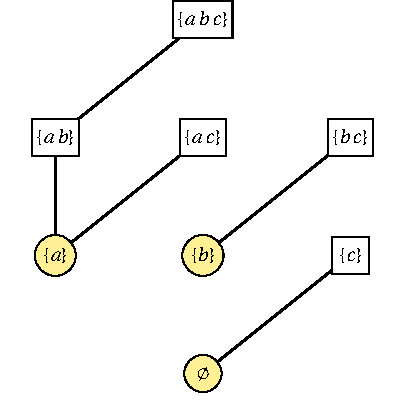
\includegraphics[clip=true]{pfs/obdd/lattice.pdf}}
     \label{fig:pfs:obdd:A} }
    & 
      \subfigure[] {\scalebox{.9}{
    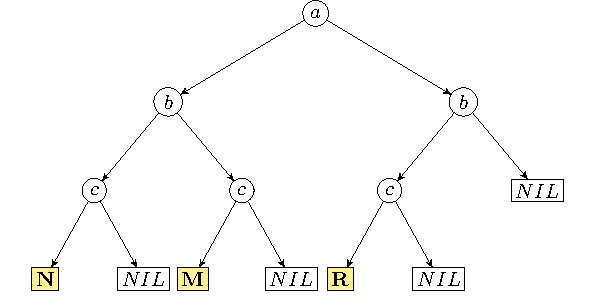
\includegraphics[clip=true]{pfs/obdd/obdd.pdf}}
    \label{fig:pfs:obdd:B} }
  \end{tabular}
    \caption{Exemplo de OBDD que representa uma floresta do 
    \algname{PFS}. Esta OBDD contém os nós $\pfsnode{N}$, $\pfsnode{M}$
    e $\pfsnode{R}$, que representam respectivamente os subconjuntos
    $000$, $010$ e $100$. As folhas $NIL$ indicam que os subconjuntos 
    de tal caminho na OBDD não são raízes na floresta, como por exemplo 
    os subconjuntos $11X$}
  \label{fig:pfs:obdd} 
\end{figure}

\subsection{Escolha de raiz}
Ao deixar de utilizar a estrutura de \toolname{map} como era feito na
implementação original do \algname{PFS}, precisamos definir uma regra
para escolha de raízes. Decidimos utilizar a regra de escolha aleatória
de raízes, dado que ela se mostrou semanticamente equivalente a
implementação original (veja \ref{pfs:root_choosing:experiments}).

Para escolher uma raiz em uma OBDD precisamos apenas descer um caminho
da raiz até uma folha não vazia (que contenha um nó) guardando os 
elementos que pertencem ao subconjunto que o caminho representa. A nossa
estrutura sempre contrai folhas redundantes para apenas uma, ou seja, não existem 
vértices na árvore que possuam dois filhos que são folhas vazias, 
portanto ao descer um caminho pela árvore, é sempre possível escolher 
a ramificação (ir a direita ou esquerda de um nó) que nos leve a uma
folha com um nó (Algoritmo~\ref{alg:Get-OBDD-Node}). 

\begin{algorithm}[]
\textsc{Get-OBDD-Node} $(X)$
\begin{algorithmic}[1]
    \State $v \gets root$
    \While{$v$ não é folha}
        \If{$v.\varname{element} \in X$}
            \State $v \gets v.\varname{right\_child}$
        \Else
            \State $v \gets v.\varname{left\_child}$
        \EndIf
    \EndWhile
    \Return $v.\varname{node}$
\end{algorithmic}
\caption{Pseudo-código de uma função que recebe um conjunto $X \in \powerset{S}$
e devolve o nó que representa este conjunto, se estiver na árvore.}
\label{alg:Get-OBDD-Node}
\end{algorithm}

Desta maneira a escolha da raiz é feita por uma sequência de escolhas
de ramificação, para cada vértice da OBDD visitado, que levam da raiz
da OBDD até um nó que é folha. Para fazer isto de maneira aleatória e
identicamente distribuída entre os nós das folhas, basta armazenar em
cada vértice da árvore quantas raízes estão a sua direita e quantos 
estão a sua esquerda e então dar pesos de escolhas equivalentes a
quantidade de raízes para cada lado de ramificação (Algoritmo~\ref{alg:Get-Random-OBDD-Node}).

\begin{algorithm}[]
\textsc{Get-Random-OBDD-Node} $()$
\begin{algorithmic}[1]
    \State $v \gets root$
    \While{$v$ não é folha}
        \State $W \gets v.\varname{right\_child}.\varname{weight} + v.\varname{left\_child}.\varname{weight}$
        \State seja $r$ um número aleatório entre 0 e $W$
        \If{$r \leq v.\varname{right\_child}.\varname{weight}$}
            \State $v \gets v.\varname{right\_child}$
        \Else
            \State $v \gets v.\varname{right\_child}$
        \EndIf
    \EndWhile
    \Return $v.\varname{node}$
\end{algorithmic}
\caption{Pseudo-código de uma função que devolve um nó aleatório da floresta
de maneira identicamente provável.}
\label{alg:Get-Random-OBDD-Node}
\end{algorithm}

\subsection{Testes com instâncias artificiais}
Testamos experimentalmente esta variação do \algname{PFS} que usa OBDDs no controle
das florestas. Vamos analisar o desempenho desta variação quanto ao tempo de execução e número de chamadas da função de custo.

Como podemos ver na tabela \ref{tab:opfs_vs_pfs}, o número de chamadas
da função de custo do algoritmo modificado é similar ao do 
\algname{PFS}, o que indica que ambos são semanticamente equivalentes; o 
que já tinha sido constatado na variante do \algname{PFS} que também
escolhia raízes aleatoriamente, mas usando \toolname{map} para controle
de floresta. Entretanto, a tabela também mostra que o tempo de execução
da modificação é maior do que do algoritmo original. Desta maneira, o
uso de OBDDs para o controle das florestas não foi vantajoso.

\begin{table}
\centering
\footnotesize
\caption{Comparação entre os algoritmos \algname{PFS} e \algname{OPFS}. 
O número de chamadas médio da função custo é parecido enquanto o tempo
de execução é maior para o \algname{OBDD}.}
\label{tab:opfs_vs_pfs}
\begin{tabular}{cc c cc c cc}
\toprule
\multicolumn{2}{c}{Instância} & \phantom{} & \multicolumn{2}{c}{Tempo de execução médio (s)}  & \phantom{} & \multicolumn{2}{c}{Número médio de cálculos de custo}\\
\cline{1-2}\cline{4-5}\cline{7-8}\\
$|S|$ & $2^{|S|}$ && PFS & OPFS && PFS & OPFS \\
10 &    1024 &&  0.013 $\pm$ 0.003 & 0.018 $\pm$ 0.003 &&  598.0 $\pm$ 192.8 & 635.5 $\pm$ 171.9 \\
11 &    2048 &&  0.020 $\pm$ 0.004 & 0.029 $\pm$ 0.007 &&  1152.1 $\pm$ 314.7 & 1117.9 $\pm$ 336.4 \\
12 &    4096 &&  0.031 $\pm$ 0.010 & 0.049 $\pm$ 0.013 &&  2024.1 $\pm$ 751.6 & 2048.2 $\pm$ 700.9 \\
13 &    8192 &&  0.057 $\pm$ 0.017 & 0.097 $\pm$ 0.033 &&  3996.3 $\pm$ 1431.6 & 3973.4 $\pm$ 1462.6 \\
14 &   16384 &&  0.094 $\pm$ 0.038 & 0.171 $\pm$ 0.063 &&  6634.8 $\pm$ 2944.0 & 6906.5 $\pm$ 2786.5 \\
15 &   32768 &&  0.182 $\pm$ 0.079 & 0.323 $\pm$ 0.156 &&  13140.1 $\pm$ 6020.6 & 12711.2 $\pm$ 6319.7 \\
16 &   65536 &&  0.370 $\pm$ 0.169 & 0.660 $\pm$ 0.314 &&  25658.2 $\pm$ 11606.7 & 25303.4 $\pm$ 12169.5 \\
17 &  131072 &&  0.819 $\pm$ 0.370 & 1.480 $\pm$ 0.665 &&  53344.9 $\pm$ 24350.4 & 53217.2 $\pm$ 24154.5 \\
18 &  262144 &&  1.515 $\pm$ 0.905 & 2.736 $\pm$ 1.626 &&  94677.6 $\pm$ 54496.3 & 94079.4 $\pm$ 55435.6 \\
19 &  524288 &&  2.612 $\pm$ 1.869 & 4.818 $\pm$ 3.355 &&  156150.5 $\pm$ 107369.8 & 156021.8 $\pm$ 107516.8 \\
20 & 1048576 &&  6.085 $\pm$ 3.900 & 11.550 $\pm$ 7.661 &&  344144.1 $\pm$ 212627.1 & 343229.2 $\pm$ 212624.4 \\
% 21 & 2097152 &&  11.416 $\pm$ 8.296 & 21.818 $\pm$ 16.269 &&  616936.2 $\pm$ 436491.2 & 613526.2 $\pm$ 438580.0 \\
% 22 & 4194304 &&  19.950 $\pm$ 17.799 & 42.112 $\pm$ 45.109 &&  960842.2 $\pm$ 785137.2 & 959905.4 $\pm$ 783257.3 \\
% 23 & 8388608 &&  42.792 $\pm$ 35.622 & 87.262 $\pm$ 90.579 &&  2053472.4 $\pm$ 1690882.1 & 2060184.5 $\pm$ 1682011.0 \\
% 24 & 16777216 &&  85.646 $\pm$ 79.186 & 149.567 $\pm$ 108.104 &&  4080290.8 $\pm$ 3166258.4 & 4100480.6 $\pm$ 3141423.9 \\
\bottomrule 
\end{tabular}%
\end{table}

\section{Paralelização do código}
A dinâmica do algoritmo \algname{Poset-Forest-Search} transforma o
reticulado Booleano em uma floresta, ou seja, em um conjunto de árvores
que são disjuntas. Por isso, o percorrimento destas árvores pode ser
feito de maneira paralela sem interferências. Desta maneira, propomos
uma paralelização do código de Reis utilizando a biblioteca 
\toolname{OpenMP}, que nos permite paralelizar blocos de instrução
com anotações feitas ao compilador.

O primeiro ponto que devemos nos atentar ao paralelizar este código é
que as árvores do espaço de busca são disjuntas apenas se estamos 
considerando uma floresta. Ambas florestas representam o mesmo espaço de
busca, portanto é possível que duas árvores de florestas diferentes se 
intersectem em alguns nós. Isto significa que fazer o percorrimento em
ambas as direções pode causar recálculos, isto é, um nó pode ser 
visitado desnecessariamente por mais de uma thread por mais de uma vez;
além disso, é possível que uma árvore que foi podada em uma direção 
ainda esteja sendo percorrida em outra direção.

Visando simplificar o trabalho, definimos que a paralelização ocorre em
iterações do procedimento principal do \algname{PFS}. Assim, a escolha
de uma direção deve ser feita por uma thread principal e, assim cada
thread deve escolher uma raiz para ser percorrida em tal direção. Desta
maneira cada thread faz a ramificação e atualização da floresta dual
e pausam em uma barreira, que sincroniza todas as threads para o 
finalização da iteração e começo da próxima.

\begin{figure}[!ht]
  \centering 
  \begin{tabular}{c c}
    \subfigure[] {\scalebox{.6}{
    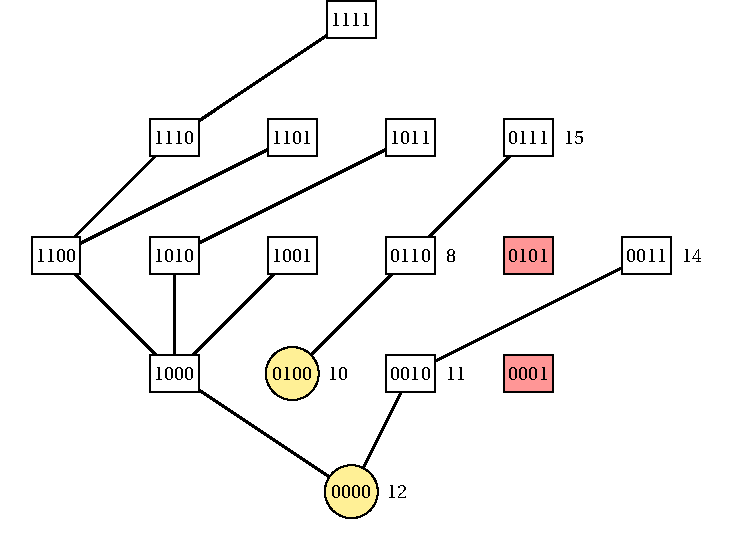
\includegraphics[clip=true]{pfs/race_cond/raceA.pdf}}
    \label{fig:pfs:race_cond:A} }
    & 
    \subfigure[] {\scalebox{.6}{
    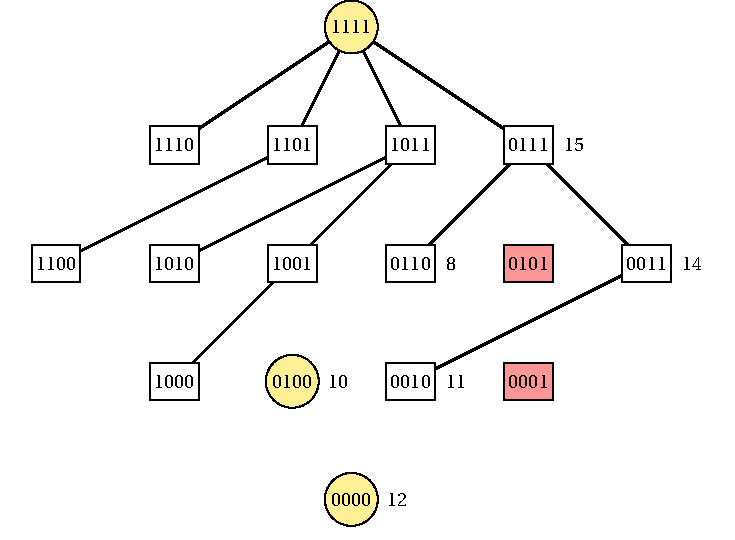
\includegraphics[clip=true]{pfs/race_cond/raceB.pdf}}
    \label{fig:pfs:race_cond:B} } \\
  \end{tabular}
  \caption{Exemplo de espaço de busca do \algname{PFS}; a floresta da
    figura~\ref{fig:pfs:race_cond:A} é $\forest_A$ enquanto a da figura~\ref{fig:pfs:race_cond:B} é $\forest_B$. Estas florestas 
    representam o espaço de busca após duas iterações do algoritmo, 
    ambas feitas na direção de baixo para cima, ou seja, ramificando
    a floresta $\forest_A$. Na primeira iteração, seleciona-se a raiz
    $0000$ para percorrimento e remove-se o nó $0001$; na floresta dual,
    a atualização remove o nó $0001$ e cria a raiz $0000$. Na segunda 
    iteração, escolhe-se novamente a raiz $0000$ e a ramificação é feita 
    para $0100$ (que se torna raiz) e para $0101$, que é removido do 
    espaço; na floresta dual, remove-se o nó $0101$ e o nó $0100$ 
    torna-se raiz.}
  \label{fig:pfs:race_cond:part1} 
\end{figure}

Entretanto, apesar desta simplificação tornar a fase de ramificação 
quase independente entre as linhas de processamento, a fase de 
atualização de floresta dual pode não ser. Como resultado, condições de
corrida não tratadas podem causar inconsistências na atualização da 
floresta. As figuras~\ref{fig:pfs:race_cond:part1}--\ref{fig:pfs:race_cond:part2} mostram
um exemplo onde duas linhas de execução podem causar este tipo de 
inconsistência. A figura~\ref{fig:pfs:race_cond:part1} mostra o 
espaço de busca do \algname{PFS} no começo de uma iteração, enquanto as
figuras~\ref{fig:pfs:race_cond:C}--\ref{fig:pfs:race_cond:D} e~\ref{fig:pfs:race_cond:E}--\ref{fig:pfs:race_cond:F} mostram 
respectivamente os resultados ao fim de uma iteração para duas 
diferentes escolhas de raízes. Na figura~\ref{fig:pfs:race_cond:D}, 
que mostra a floresta $\forest_B$ quando a raiz escolhida é $0100$,
o nó $0111$ é removido do espaço de busca; na figura~\ref{fig:pfs:race_cond:F}, que mostra a floresta $\forest_B$ quando a 
raiz escolhida é $0000$, o nó $0111$ torna-se raiz. Assuma então que
esta iteração do algoritmo é feita com duas linhas de processamento 
$P_1$ e $P_2$, que fazem o percorrimento, respectivamente, a partir de 
$0000$ e $0100$. Se a thread $P_1$ cria o nó $0111$ antes de $P_2$ 
removê-lo, então não há inconsistências, entretanto se o contrário
acontece, criamos uma raiz espúria na floresta $\forest_B$.

\begin{figure}[!ht]
  \centering 
  \begin{tabular}{c c}
    \subfigure[] {\scalebox{.6}{
    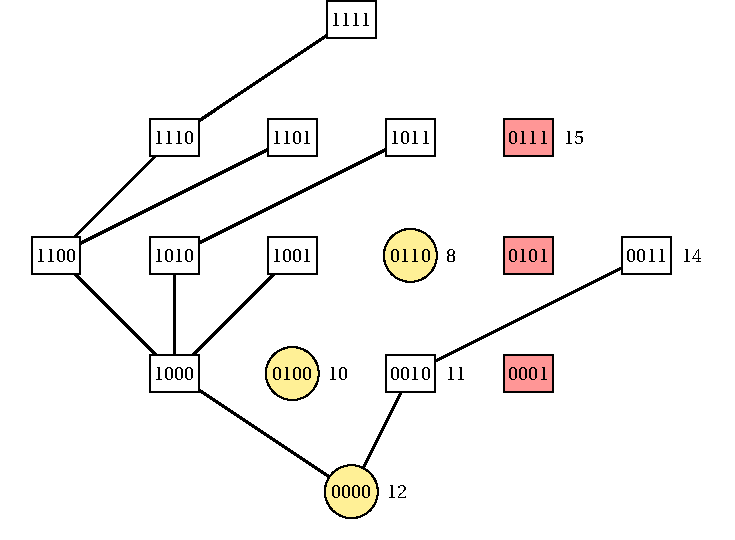
\includegraphics[clip=true]{pfs/race_cond/raceC.pdf}}
    \label{fig:pfs:race_cond:C} }
    & 
    \subfigure[] {\scalebox{.6}{
    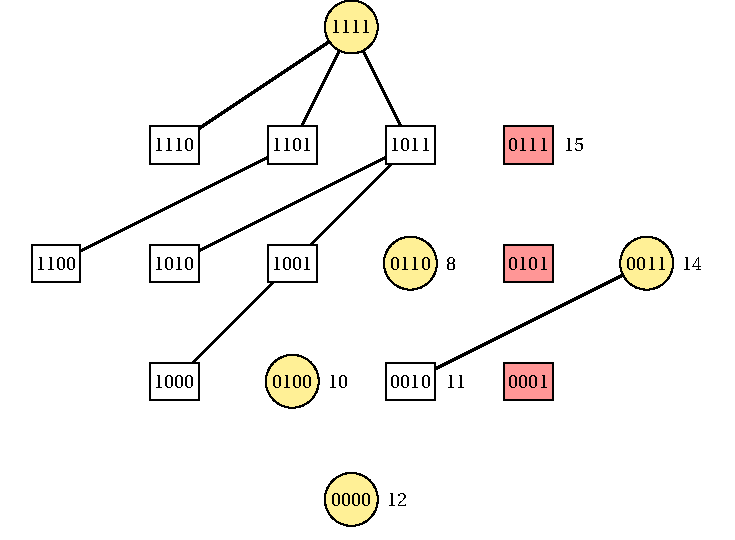
\includegraphics[clip=true]{pfs/race_cond/raceD.pdf}}
    \label{fig:pfs:race_cond:D} } \\
    \subfigure[] {\scalebox{.6}{
    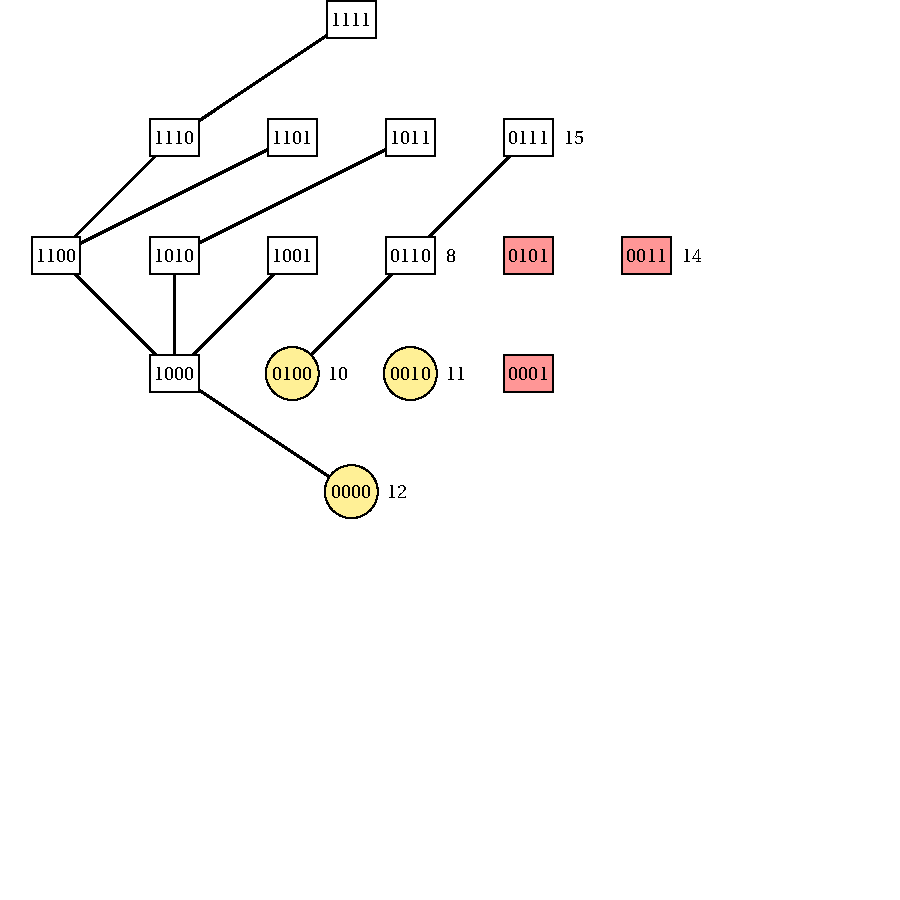
\includegraphics[clip=true]{pfs/race_cond/raceE.pdf}}
    \label{fig:pfs:race_cond:E} }
    & 
    \subfigure[] {\scalebox{.6}{
    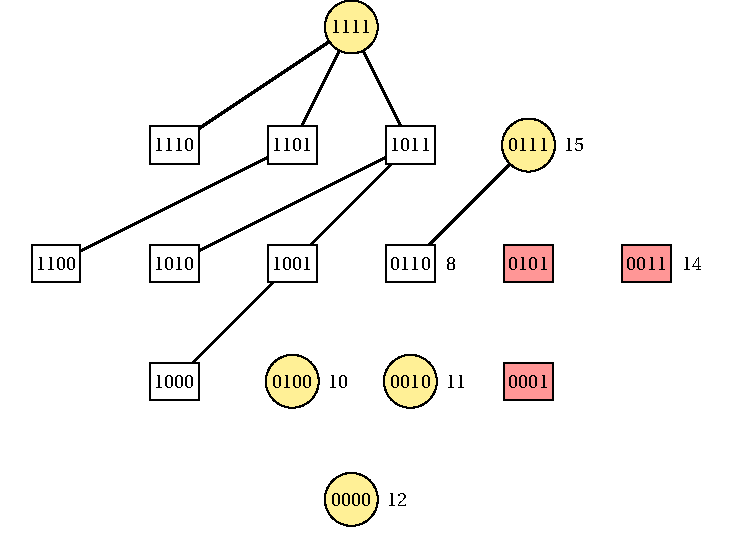
\includegraphics[clip=true]{pfs/race_cond/raceF.pdf}}
    \label{fig:pfs:race_cond:F} } \\
  \end{tabular}
  \caption{Continuação do exemplo da figura~\ref{fig:pfs:race_cond:part1} para duas escolhas diferentes de 
    raízes. As figuras~\ref{fig:pfs:race_cond:C} e~\ref{fig:pfs:race_cond:D} mostram o resultado da continuação da 
    execução do algoritmo após escolha da raiz $0100$ de $\forest_A$ em 
    um percorrimento de baixo para cima que ramifica até o nó 
    $0111$, que é podado da floresta $\forest_A$; na floresta dual, o nó
    $0111$ é removido e os nós $0110$ e $0011$ tornam-se raízes. As 
    figuras~\ref{fig:pfs:race_cond:E} e~\ref{fig:pfs:race_cond:F} 
    mostram a continuação da execução quando a raiz $0000$ de 
    $\forest_A$ é escolhida para percorrimento, que ramifica até o nó
    $0011$, que é podado da floresta $\forest_A$; na floresta dual, o nó
    $0011$ é removido e o nó $0010$ torna-se raiz.} 
  \label{fig:pfs:race_cond:part2} 
\end{figure}

Para contornar este problema, utilizamos uma outra estrutura de dados
do \langname{C++} capaz de armazenar um conjunto. Neste conjunto 
armazenamos todos os nós que foram removidos do espaço de busca em uma
iteração e assim evitamos a criação de raízes espúrias. Note que esse 
conjunto é esvaziado a cada iteração do \algname{PFS}, portanto não
deve ocupar grande espaço de memória; se este conjunto não fosse limpo
a cada iteração ele poderia atingir tamanhos exponenciais sobre o número
de características do problema, comprometendo a escalabilidade do 
algoritmo.


Voltando ao exemplo anterior, das figuras~\ref{fig:pfs:race_cond:part1}--\ref{fig:pfs:race_cond:part2}, com a 
criação do conjunto de nós deletados, se a linha de processamento $P_1$
deleta o nó $0111$ antes da criação em $P_2$, então o nó já estará no 
conjunto de nós deletados quando $P_2$ tentar adicioná-lo na floresta e
assim a criação desta raiz pode ser evitada. Se a ordem é contrária, 
então o nó é criado e depois deletado, o que pode ser desnecessário, 
porém consistente.

\subsection{Testes com instâncias artificiais}
Testamos experimentalmente esta versão paralela do \algname{PFS}, que chamamos aqui de
\algname{PPFS}. Vamos agora analisar o desempenho 
deste algoritmo quanto ao tempo de execução e número de chamadas da 
função de custo.

\begin{table}
\centering
\footnotesize
\caption{Comparação entre os algoritmos \algname{PFS} e \algname{PPFS}.
O algoritmo \algname{PPFS} apresenta um número similar de média de 
chamadas da função custo ao \algname{PFS}, mas possui tempo de execução 
médio maior.}
\label{tab:ppfs_vs_pfs}
% \resizebox{\columnwidth}{!}{%
\begin{tabular}{cc c cc c cc}
\toprule
\multicolumn{2}{c}{Instância} & \phantom{} & \multicolumn{2}{c}{Tempo de execução médio (s)} & \phantom{} & \multicolumn{2}{c}{Número médio de cálculos de custo} \\
\cline{1-2}\cline{4-5}\cline{7-8}\\
$|S|$ & $2^{|S|}$ && PFS & PPFS && PFS & PPFS \\
 % 1 &       2 && 0.005 $\pm$ 0.004 & 0.028 $\pm$ 0.006 &&  2.0 $\pm$  0.0 &  2.0 $\pm$  0.0 \\
 % 2 &       4 && 0.004 $\pm$ 0.000 & 0.038 $\pm$ 0.008 &&  3.9 $\pm$  0.3 &  3.9 $\pm$  0.3 \\
 % 3 &       8 && 0.004 $\pm$ 0.000 & 0.039 $\pm$ 0.007 &&  7.0 $\pm$  1.2 &  7.0 $\pm$  1.2 \\
 % 4 &      16 && 0.004 $\pm$ 0.000 & 0.047 $\pm$ 0.008 && 12.8 $\pm$  3.0 & 13.2 $\pm$  3.3 \\
 % 5 &      32 && 0.005 $\pm$ 0.000 & 0.058 $\pm$ 0.009 && 26.8 $\pm$  4.5 & 26.9 $\pm$  3.0 \\
 % 6 &      64 && 0.005 $\pm$ 0.000 & 0.061 $\pm$ 0.010 && 52.7 $\pm$  7.3 & 50.5 $\pm$  6.4 \\
 % 7 &     128 && 0.005 $\pm$ 0.000 & 0.070 $\pm$ 0.013 && 87.3 $\pm$ 20.5 & 82.8 $\pm$ 23.5 \\
 % 8 &     256 && 0.006 $\pm$ 0.000 & 0.079 $\pm$ 0.013 && 177.0 $\pm$ 32.1 & 171.2 $\pm$ 36.2 \\
 % 9 &     512 && 0.008 $\pm$ 0.001 & 0.104 $\pm$ 0.021 && 333.8 $\pm$ 93.9 & 344.5 $\pm$ 95.2 \\
10 &    1024 && 0.011 $\pm$ 0.001 & 0.146 $\pm$ 0.027 && 643.6 $\pm$ 133.0 & 626.5 $\pm$ 151.1 \\
11 &    2048 && 0.017 $\pm$ 0.004 & 0.227 $\pm$ 0.062 && 1151.0 $\pm$ 359.7 & 1135.6 $\pm$ 381.1 \\
12 &    4096 && 0.029 $\pm$ 0.007 & 0.385 $\pm$ 0.113 && 2173.1 $\pm$ 652.5 & 2139.2 $\pm$ 710.3 \\
13 &    8192 && 0.049 $\pm$ 0.015 & 0.640 $\pm$ 0.237 && 3839.8 $\pm$ 1376.6 & 3743.5 $\pm$ 1532.9 \\
14 &   16384 && 0.104 $\pm$ 0.037 & 1.337 $\pm$ 0.513 && 8175.9 $\pm$ 3037.4 & 8026.4 $\pm$ 3303.7 \\
15 &   32768 && 0.163 $\pm$ 0.078 & 2.010 $\pm$ 1.096 && 12459.6 $\pm$ 6164.5 & 12062.2 $\pm$ 6897.2 \\
16 &   65536 && 0.360 $\pm$ 0.163 & 4.483 $\pm$ 2.030 && 27027.3 $\pm$ 12397.0 & 26835.7 $\pm$ 12446.9 \\
17 &  131072 && 0.664 $\pm$ 0.362 & 8.072 $\pm$ 4.370 && 48001.9 $\pm$ 26149.2 & 48093.4 $\pm$ 26233.2 \\
18 &  262144 && 1.250 $\pm$ 0.690 & 14.341 $\pm$ 8.062 && 85880.9 $\pm$ 47950.8 & 86050.8 $\pm$ 49186.8 \\
19 &  524288 && 2.936 $\pm$ 1.629 & 34.639 $\pm$ 19.074 && 198503.0 $\pm$ 108116.1 & 197832.5 $\pm$ 110659.6 \\
20 & 1048576 && 5.024 $\pm$ 3.097 & 61.038 $\pm$ 38.250 && 321495.8 $\pm$ 198004.3 & 318507.0 $\pm$ 199354.3 \\
% 21 & 2097152 && 11.997 $\pm$ 7.637 & 144.610 $\pm$ 89.521 && 754636.3 $\pm$ 478683.6 & 759129.7 $\pm$ 472831.1 \\
\bottomrule
\end{tabular}
% }
\end{table}

Podemos observar na tabela~\ref{tab:ppfs_vs_pfs} que os números de 
chamadas da função custo dos algoritmos \algname{PFS} e \algname{PPFS}
são parecidos. Isto quer dizer que a nossa paralelização não trouxe 
grandes modificações semânticas ao algoritmo. Entretanto, o tempo médio
de execução teve diferenças na versão paralela, que gastou mais tempo
do que o algoritmo original em todas as instâncias. A tabela mostra
que o \algname{PPFS} foi pelo menos 10 vezes mais lento que a 
implementação serial para as instâncias vistas.


\subsection{Comentários sobre experimentos}
Acreditamos que os resultados pobres do algoritmo \algname{PPFS} se 
deram por conta da complexidade da atualização da floresta dual. 
Apesar das ramificações serem feitas em paralelo com pouco ou nenhum
entrelace de linhas de processamento, esta rotina consome tempo de
execução pequeno comparado com a rotina de atualização de florestas.
Com a paralelização, esta atualização tornou necessária uma nova 
estrutura de dados ao algoritmo para tratar condições de corrida 
que podiam adicionar inconsistências as florestas. Além disso, a 
atualização depende de adições, remoções e verificações nas 
florestas que não podem ser feitas em paralelo, criando muitas seções
críticas no código, o que deve ter sido a principal causa da piora
de tempo, pois estes blocos de código implicam em uma troca constante
de contextos pelos processadores, que não podem processar blocos
críticos ao mesmo tempo.

\section{O algoritmo UBB-PFS}
\label{sec:ubbpfs}
Tendo em vista que o principal problema da paralelização do 
$\algname{PFS}$ foi o fato de que há muito entrelace nas linhas de 
execução, propomos um novo algoritmo baseado no $\algname{UBB}$ e 
$\algname{PFS}$ que fosse também paralelo, mas com pouca ou nenhuma 
interferência entre as linhas de execução, chamamos este algoritmo de 
\algname{UBB-PFS}.

\subsection{Descrição}
Este algoritmo tem duas etapas principais. A primeira etapa é idêntica
ao \algname{UBB}, e faz o percorrimento de uma árvore do espaço de busca
como em uma busca em profundidade, podando os nós em que o custo cresce.
Depois de um certo número de iterações, a primeira etapa é finalizada e 
então se dá início a segunda etapa, que deve resolver cada sub-árvore 
do espaço de busca corrente utilizando o algoritmo \algname{PFS}. A 
solução das sub-árvores deve ocorrer de maneira independente, 
possibilitando a paralelização mais fácil do código.

O pseudo-código do algoritmo~\ref{pfs:code:ubbpfs:step1} mostra como é feita a 
primeira etapa do algoritmo e também serve de base para a explicação da
segunda etapa \algname{UBB-PFS} e da corretude do algoritmo, pois 
possui os seguintes invariantes no final da linha~\ref{pfs:code:ubbpfs:invariant}:
\begin{enumerate}[a)]
    \item{Para todo nó do espaço de busca que não é raiz, existem três 
        possibilidades: ou ele foi visitado e está em $\mathcal{M}$, ou 
        podado, ou e está contido em uma sub-árvore tal que a raiz está 
        na pilha $\mathcal{S}$. Todo nó que é raiz está em 
        $\mathcal{M}$}; \label{pfs:code:ubb:invariant:A}
    \item{Todo nó na pilha $\mathcal{S}$ é raiz de uma sub-árvore 
        completa.} \label{pfs:code:ubb:invariant:B}
\end{enumerate}

\begin{algorithm}[!ht]
\textsc{UBB-PFS} $(S, c)$
\begin{algorithmic}[1]
    \State $\mathcal{M} \gets \emptyset$
    \State inicialize a pilha $\mathcal{S}$ vazia
    \State empilhe $(\emptyset, S, c(\emptyset))$ em $\mathcal{S}$
    \While{$\mathcal{S}$ não vazia} \label{pfs:code:ubbpfs:step1:A}
        \State desempilhe $(Y, X, cost_Y)$ de $\mathcal{S}$
        \State $X_{Y_i} \gets \emptyset$
        \While{$X \ne \emptyset$} 
            \State remova $s_i$ de $X$
            \State $Y_i \gets Y \cup \{s_i\}$
            \State $cost_{Y_i} \gets c (Y_i)$
            \If{$cost_{Y_i} \leq cost_Y$}
                \State empilhe $(Y_i, X_{Y_i}, cost_{Y_i})$ em $\mathcal{S}$
            \EndIf
            \State $X_{Y_i} \gets {s_i}$
        \EndWhile
        \State $\mathcal{M} \gets \mathcal{M} \cup \{Y\}$ \label{pfs:code:ubbpfs:invariant}
        \If{$\mathsc{FinishStepOne} ()$}
            \State $\mathcal{N} \gets \mathsc{SolveTrees} (\mathcal{S}, S, c)$
            \State esvazie $\mathcal{S}$
        \EndIf
    \EndWhile \label{pfs:code:ubbpfs:step1:B}
    \State $\mathcal{M} \gets \mathcal{M} \cup \mathcal{N}$
    \Return $\{M \in \mathcal{M} : c(M) \text{é mínimo}\}$
\end{algorithmic}
\caption{Pseudo-código do algoritmo \algname{UBB-PFS}. A primeira etapa 
consiste no percorrimento feito nas linhas 
\ref{pfs:code:ubbpfs:step1:A}~-~\ref{pfs:code:ubbpfs:step1:B}, de 
maneira idêntica ao \algname{UBB}.}
\label{pfs:code:ubbpfs:step1}
\end{algorithm}


O invariante~\ref{pfs:code:ubb:invariant:A} nos garante que o mínimo
global já está em $\mathcal{M}$ ou é minimo dentro de uma das árvores
que tem raiz em $\mathcal{S}$, portanto, quando estamos na linha do 
invariante, resolver o problema original é igual a achar o mínimo
de cada uma das árvores e do conjunto $\mathcal{M}$. O 
invariante~\ref{pfs:code:ubb:invariant:B} garante que toda árvore com 
raiz $Y$ contém exatamente os subconjuntos do intervalo $[Y, X \cup Y]$. 

Para resolver cada sub-árvore com raiz em $\mathcal{S}$, criamos o 
seguinte problema U-curve auxiliar. Seja $\langle S, c \rangle$ uma 
instância do problema U-curve e seja $Y$ uma raiz de uma sub-árvore do 
problema e $X$ um conjunto de características tal que os nós desta 
sub-árvore seja exatamente o intervalo $[Y, X \cup Y]$. Considerando que
este intervalo é igual ao conjunto $\{Y \cup W : W \in \powerset(X)\}$,
então, encontrar o mínimo dentro deste conjunto é exatamente resolver a 
instância do problema U-curve $\langle S_X, c_Y\rangle$ tal que:
\begin{subequations}
\begin{alignat*}{2}
    S_X      & = X & \\
    c_Y (X') & = c (X' \cup Y) & \text{, } ~X' \in \powerset(S_X).
\end{alignat*}
\end{subequations}
Cada uma dessas instâncias é resolvida utilizando a função \algname{SolveTrees} (Algoritmo~\ref{alg:Solve-Trees}).
\begin{algorithm}[!ht]
\textsc{SolveTrees}$(\mathcal{S}, S, c)$
\begin{algorithmic}[1]
    \State $\mathcal{N} \gets \emptyset$
    \While{$\mathcal{S}$ não vazia}
        \State desempilhe $(Y, X, cost_Y)$
        \State $S_X \gets X$
        \State seja $c_Y: X' \mapsto c (X' \cup Y)$
        \State $N \gets \mathsc{Poset-Forest-Search} (S_X, c_Y)$
        \State $\mathcal{N} \gets \mathcal{N} \cup N$
    \EndWhile
    \Return $\mathcal{N}$
\end{algorithmic}
\caption{Pseudo-código da função \algname{SolveTrees}.}
\label{alg:Solve-Trees}
\end{algorithm}

A função \textsc{FinishStepOne} determina qual é a iteração em que o
algoritmo deve terminar a primeira etapa. Esta função Booleana controla,
de certa forma, a maneira com que o trabalho é dividido entre etapa 1 e 
2 do código. Se ela nunca for verdadeira, então o \algname{UBB-PFS} deve 
se comportar exatamente como o \algname{UBB}. Além disso, a segunda 
etapa deve ser rodada em linhas de processamento paralelos, portanto
esta função também influencia a distribuição de trabalho e nível de 
paralelização.

\subsection{Paralelização}
A paralelização deste algoritmo também foi feita com a biblioteca 
\toolname{OpenMP}. Conseguimos paralelizar este código com apenas 
algumas anotações para o compilador, que indicam que a função
\textsc{SolveTrees} deve criar tarefas (\foreignword{tasks}) para cada 
chamada do algoritmo \textsc{Poset-Forest-Search}, e também que deve 
haver uma barreira que só permite o retorno da função 
\textsc{SolveTrees} quando todas as tarefas criadas foram resolvidas.

Para que a paralelização traga melhoras significativas é esperado que
haja um número razoável de árvores na pilha $\mathcal{S}$. Um exemplo de
número de raízes que é razoável para paralelização é a quantidade de
processadores da máquina. A função \textsc{FinishStepOne} deve garantir
que terminamos a primeira etapa do \algname{UBB-PFS} com um número
razoável de raízes na pilha. Note que o número de raízes é limitado
pela própria topologia do problema; se a função é, por exemplo, monótona
crescente, então a única raiz empilhada é a do conjunto vazio.

Em nossa implementação, definimos que a função \textsc{FinishStepOne} é
verdadeira quando o número de raízes é maior que o número de cores da 
máquina ou quando o número de iterações é maior do que duas vezes a 
quantidade de características. 

\subsection{Experimentos com instâncias artificiais}
Testamos o algoritmo \algname{UBB-PFS} em experimentos computacionais. Analisaremos agora o desempenho dos algoritmos tanto quanto ao 
tempo médio de execução quanto a quantidade de nós computados.

A tabela~\ref{tab:ubbpfs_vs_ubb_vs_pfs_time} mostra o tempo de execução
dos algoritmos \algname{PFS}, \algname{UBB-PFS} e \algname{UBB}. O 
\algname{UBB-PFS} teve tempos de execuções médios menores do que o 
\algname{PFS}, portanto precisamos investigar se ele é melhor também do
que um outro algoritmo mais rápido que o \algname{PFS}, o \algname{UBB}.
Este último mostrou ter melhor desempenho nesta tabela, entretanto, 
por conta da paralelização, é possível que o \algname{UBB-PFS} se torne 
mais rápido para instâncias maiores. Investigamos isto com instâncias
maiores na tabela~\ref{tab:ubbpfs_vs_ubb_time} e constatamos que 
para estas instâncias o \algname{UBB} ainda é mais rápido.

A tabela~\ref{tab:ubbpfs_vs_ubb_vs_pfs_computed_nodes} mostra o número
médio de nós computados pelos mesmos algoritmos. Podemos observar nesta
tabela que o \algname{UBB}, apesar de ser mais rápido, precisa computar
mais nós que os outros algoritmos. O \algname{PFS} é o algoritmo que 
precisa calcular menos nós, enquanto o \algname{UBB-PFS} é 
intermediário, mas com desempenho mais próximo do \algname{PFS}.

\subsection{Comentários sobre os experimentos}
Dado que o tempo de execução do \algname{UBB-PFS} foi menor do que o
tempo do \algname{PFS} e que o número de nós computados foi menor do
que o necessário pelo \algname{UBB}, que é o mais rápido dos três, 
concluímos que existem instâncias em que o \algname{UBB-PFS} é o 
algoritmo mais apropriado entre os três. Este tipo de instância é tal
que o tempo de percorrimento é tão relevante quanto o tempo de 
computação da função custo, desta maneira o número maior de cálculos
do \algname{UBB} e o tempo maior de percorrimento do \algname{PFS} 
tornariam o \algname{UBB-PFS} a melhor opção, porque é intermediário no 
consumo de tempo e próximo do melhor dos três quanto ao número de 
cálculos da função custo.

\begin{table}
\centering
\footnotesize
\caption{Comparação de tempo médio de execução entre os algoritmos
\algname{UBB}, \algname{PFS} e \algname{UBB-PFS}. Podemos observar que
o \algname{PFS} foi o mais lento enquanto o \algname{UBB} foi o mais
rápido e o \algname{UBB-PFS} teve desempenho itermediário para estas
instâncias. Este teste continua na tabela~\ref{tab:ubbpfs_vs_ubb_time},
que mostra apenas o \algname{UBB} e o \algname{UBB-PFS} já que o 
\algname{PFS} mostrou ter desempenho pior.}
\label{tab:ubbpfs_vs_ubb_vs_pfs_time}
% \resizebox{\columnwidth}{!}{%
\begin{tabular}{cc c ccc}
\toprule
\multicolumn{2}{c}{Instância} & \phantom{} & \multicolumn{3}{c}{Tempo de execução médio (s)}\\
\cline{1-2}\cline{4-6}\\
$|S|$ & $2^{|S|}$ && UBB & PFS & UBB-PFS  \\
10 &    1024 &&  0.006 $\pm$ 0.001 & 0.011 $\pm$ 0.002 & 0.023 $\pm$ 0.004 \\
11 &    2048 &&  0.007 $\pm$ 0.001 & 0.017 $\pm$ 0.004 & 0.026 $\pm$ 0.004 \\
12 &    4096 &&  0.010 $\pm$ 0.003 & 0.029 $\pm$ 0.009 & 0.034 $\pm$ 0.006 \\
13 &    8192 &&  0.013 $\pm$ 0.006 & 0.047 $\pm$ 0.016 & 0.044 $\pm$ 0.011 \\
14 &   16384 &&  0.024 $\pm$ 0.013 & 0.094 $\pm$ 0.034 & 0.068 $\pm$ 0.023 \\
15 &   32768 &&  0.043 $\pm$ 0.026 & 0.186 $\pm$ 0.074 & 0.113 $\pm$ 0.042 \\
16 &   65536 &&  0.083 $\pm$ 0.060 & 0.339 $\pm$ 0.168 & 0.187 $\pm$ 0.082 \\
17 &  131072 &&  0.161 $\pm$ 0.122 & 0.650 $\pm$ 0.347 & 0.326 $\pm$ 0.175 \\
18 &  262144 &&  0.321 $\pm$ 0.233 & 1.482 $\pm$ 0.768 & 0.703 $\pm$ 0.380 \\
19 &  524288 &&  0.620 $\pm$ 0.447 & 2.711 $\pm$ 1.562 & 1.309 $\pm$ 0.729 \\
20 & 1048576 &&  1.312 $\pm$ 0.970 & 5.007 $\pm$ 3.302 & 2.478 $\pm$ 1.547 \\
21 & 2097152 &&  2.494 $\pm$ 1.893 & 11.125 $\pm$ 6.749 & 5.458 $\pm$ 3.294 \\
22 & 4194304 &&  4.589 $\pm$ 4.122 & 19.085 $\pm$ 15.147 & 8.832 $\pm$ 6.846 \\
23 & 8388608 &&  12.228 $\pm$ 7.922 & 40.323 $\pm$ 29.649 & 18.891 $\pm$ 12.786 \\
24 & 16777216 &&  24.273 $\pm$ 16.277 & 113.332 $\pm$ 76.688 & 67.178 $\pm$ 46.516 \\
\bottomrule
\end{tabular}
% }
\end{table}

\begin{table}
\centering
\footnotesize
\caption{Comparação de tempo médio de execução entre os algoritmos 
\algname{UBB} e \algname{UBB-PFS}. O algoritmo \algname{UBB-PFS} mostrou
maior tempo médio de execução.}
\label{tab:ubbpfs_vs_ubb_time}
\begin{tabular}{cc c cc}
\toprule
\multicolumn{2}{c}{Instância} & \phantom{} & \multicolumn{2}{c}{Tempo de execução médio (s)} \\
\cline{1-2}\cline{4-5}\\
$|S|$ & $2^{|S|}$ && UBB & UBB-PFS \\
20 & 1048576 &&  1.245 $\pm$ 0.861 & 5.106 $\pm$ 3.017 \\
21 & 2097152 &&  2.332 $\pm$ 1.900 & 9.178 $\pm$ 6.330 \\
22 & 4194304 &&  5.653 $\pm$ 3.904 & 17.405 $\pm$ 11.754 \\
23 & 8388608 &&  9.432 $\pm$ 8.938 & 28.746 $\pm$ 26.387 \\
24 & 16777216 &&  20.293 $\pm$ 16.147 & 77.392 $\pm$ 59.976 \\
25 & 33554432 &&  46.215 $\pm$ 35.837 & 144.196 $\pm$ 110.583 \\
\bottomrule
\end{tabular}
\end{table}


\begin{table}
\centering
\footnotesize
\caption{Comparação sobre o número de chamadas de função custo entre
os algoritmos \algname{UBB}, \algname{PFS} e \algname{UBB-PFS}. Vemos
nesta tabela que o número de nós computados pelo \algname{UBB} é o maior
enquanto o do \algname{PFS} é o menor; o \algname{UBB-PFS} tem 
desempenho intermediário, porém próximo ao do \algname{PFS}.}
\label{tab:ubbpfs_vs_ubb_vs_pfs_computed_nodes}
% \resizebox{\columnwidth}{!}{%
\begin{tabular}{cc c ccc}
\toprule
\multicolumn{2}{c}{Instância} & \phantom{} & \multicolumn{3}{c}{Número médio de cálculos de custo}\\
\cline{1-2}\cline{4-6} \\
$|S|$ & $2^{|S|}$ && UBB & PFS & UBB-PFS  \\
10 &    1024  && 699.4 $\pm$ 361.3 & 611.3 $\pm$ 178.8 & 634.7 $\pm$ 209.8 \\
11 &    2048  && 1217.2 $\pm$ 747.1 & 1145.4 $\pm$ 358.9 & 1178.8 $\pm$ 484.1 \\
12 &    4096  && 2898.0 $\pm$ 1380.4 & 2103.1 $\pm$ 793.6 & 2363.0 $\pm$ 760.4 \\
13 &    8192  && 4422.6 $\pm$ 3293.8 & 3650.9 $\pm$ 1371.9 & 3934.4 $\pm$ 1487.7 \\
14 &   16384  && 10089.4 $\pm$ 6452.1 & 7536.3 $\pm$ 2926.1 & 8012.2 $\pm$ 3387.4 \\
15 &   32768  && 19097.5 $\pm$ 12793.8 & 14546.5 $\pm$ 6081.0 & 15299.2 $\pm$ 6598.4 \\
16 &   65536  && 37663.1 $\pm$ 28321.2 & 25744.0 $\pm$ 12795.4 & 27028.4 $\pm$ 13031.9 \\
17 &  131072  && 73373.3 $\pm$ 55994.3 & 46808.9 $\pm$ 24533.5 & 49348.6 $\pm$ 24556.7 \\
18 &  262144  && 150035.2 $\pm$ 108299.3 & 103166.6 $\pm$ 52464.7 & 105306.4 $\pm$ 53472.0 \\
19 &  524288  && 292561.2 $\pm$ 210771.2 & 183125.7 $\pm$ 104965.4 & 189545.7 $\pm$ 102145.9 \\
20 & 1048576  && 617049.5 $\pm$ 450468.2 & 323097.4 $\pm$ 213634.3 & 340694.2 $\pm$ 202389.6 \\
21 & 2097152  && 1172641.6 $\pm$ 879148.5 & 691991.3 $\pm$ 413262.9 & 704790.2 $\pm$ 407143.8 \\
22 & 4194304  && 2099973.2 $\pm$ 1863285.8 & 1133395.1 $\pm$ 874492.0 & 1156564.2 $\pm$ 862152.0 \\
23 & 8388608  && 5435778.8 $\pm$ 3468245.3 & 2276694.5 $\pm$ 1621342.2 & 2345648.2 $\pm$ 1558258.5 \\
24 & 16777216 && 10146842.9 $\pm$ 6673018.3 & 5527504.2 $\pm$ 3413432.3 & 5609052.7 $\pm$ 3337059.1 \\
\bottomrule
\end{tabular}
% }
\end{table}


\chapter{O algoritmo Parallel U-Curve Search}
O algoritmo \algname{Parallel U-Curve Search} (PUCS) foi desenvolvido 
para resolver o problema U-Curve particionando o espaço de busca em 
partes que podem ser resolvidas independentemente e de forma paralela. 
Além disso, a dinâmica desse algoritmo depende de parâmetros que 
determinam o tempo de execução e qualidade da solução obtida, permitindo
ao usuário adequar o algoritmo aos recursos computacionais disponíveis. 

\section{Princípios do algoritmo}
 
\subsection{Partição do espaço de busca}
Seja $S$ o conjunto de características do problema em questão. O 
primeiro passo do particionamento é escolher arbitrariamente $S'$ um 
subconjunto de $S$; de maneira complementar, definimos 
$\overline{S'} = S \setminus S'$. Agora, sejam $X, Y \in \powerset (S)$
e $\sim$ a relação:

\begin{equation*}
    X \sim Y \iff (X \cap S') = (Y \cap S')
\end{equation*}
Esta relação é de equivalência, pois nela valem:

\begin{itemize}
    \item{reflexividade}
        \begin{align*} 
            X \sim X \text{, pois }
            (X \cap S') = (X \cap S')
        \end{align*} 
    \item{simetria}
        \begin{align*}
            X \sim Y  & \iff \\
            (X \cap S') = (Y \cap S') & \iff \\
            (Y \cap S') = (X \cap S') & \iff \\
            Y \sim X 
        \end{align*}
    \item{transitividade,}
        \begin{align*}
            X \sim Y, Y \sim Z & \Rightarrow \\
            (X \cap S') = (Y \cap S') = (Z \cap S') & \Rightarrow \\
            (X \cap S') = (Z \cap S') & \Rightarrow \\
            X \sim Z
        \end{align*}
\end{itemize}
Portanto, o conjunto das classes de equivalência definidas por $\sim$ é
uma partição do espaço de busca original. Tome como exemplo o conjunto
$S = \{a, b, c\}$; se $S' = {a}$, então existem duas classes de 
equivalência no particionamento do espaço de busca que definimos, 
formados pelos conjuntos $\{\emptyset, b, c, bc\}$ e $\{a, ab, ac, 
abc\}$.

Pela definição da relação $\sim$ temos que a presença de cada 
característica de $S'$ em uma dada parte do reticulado não muda, isto é,
ou ela está presente em todos subconjuntos da parte ou não está presente
em nenhum, portanto, dizemos que estas variáveis são {\bf fixas}. De 
modo análogo, as variáveis de $\overline{S'}$ são {\bf livres}. Tanto 
variáveis fixas quanto livres podem definir reticulados booleanos junto 
a relação de ordem parcial $\subseteq$.

O conjunto $\powerset (S')$ induz um reticulado booleano em que cada
elemento representa uma classe de equivalência do espaço de soluções
do problema original, chamamos este de {\bf reticulado externo}. Para 
cada classe de equivalência (nó do reticulado externo), o conjunto 
$\powerset (\overline {S'})$ induz um outro reticulado booleano ({\bf
reticulado interno}) em que cada elemento representa um subconjunto de
problema original. Seja $A \in \powerset (S')$ um elemento do reticulado 
externo, então cada $B \in \powerset (\overline{S'})$ do reticulado 
interno em $A$ representa o conjunto $X = B \cup A$ do espaço de busca
do problema original.

Os reticulados internos e externo elucidam a estrutura recursiva do 
problema de seleção de características e sugerem que podemos construir 
uma solução ao problema original a partir de soluções de outros 
problemas, sobre os reticulados externo e internos, abordagem conhecida
em computação como divisão e conquista. Seja $\langle S, c \rangle$ uma 
instância do problema de seleção de características, $S'$ o conjunto de 
variáveis fixas, $\overline{S'}$ o conjunto de variáveis livres, e 
$A \in \powerset (S')$ um subconjunto que é nó do reticulado externo, 
então podemos definir um outro problema de seleção de características 
$\langle \overline{S'}, c_{A} \rangle$ em que 
\begin{align*}
    c_{A} (X) = c (X \cup A).
\end{align*}
Resolver a instância $\langle \overline{S'}, c_{A} \rangle$ é 
essencialmente achar o mínimo do problema inicial restrito a classe de
equivalência de $A$, dizemos também que estamos resolvendo a parte $A$. 
Se soubermos em qual classe o mínimo global reside, podemos resolver 
apenas tal parte e garantir que a solução encontrada é a solução do 
problema original.

O algoritmo PUCS percorre o reticulado externo recolhendo partes 
candidatas a conter o mínimo e resolve cada uma destas, escolhendo o 
mínimo das soluções destas partes como o mínimo global do problema.

\subsection{Percorrimento do reticulado externo}


\chapter{Conclusão}
Nesta seção vamos fazer uma revisão deste trabalho, apontando e 
discutindo os resultados obtidos. Também vamos apresentar algumas opções
de linhas de pesquisa para trabalhos futuros relacionados a este.
\section{Revisão do trabalho}
% - estudamos o ubb e o pfs e com isso pudemos
%   - modificar a escolha das raízes
%     - uma escolha arbitrária parece ser melhor do que escolher uma
%       raiz que tem a maior sub-árvore.
%   - modificar estrutura de dados para escolha de raíz
%     - não foi eficiente
%   - paralelizar o PFS
%     - apesar da ramificação ser disjunta, a etapa de atualização
%       compromete o desempenho da paralelização
%   - criar um algoritmo que divide o trabalho
% - usando a ideia de dividir o trabalho, criamos o PUCS
%   - particionamento do espaço em partes iguais - melhor distribuição
%     de trabalho
%   - parâmetros que permitem controlar a granularidade do 
%     particionamento
%   - como algoritmo ótimo é mais lento que outros algoritmos
%   - como heurística acha melhores soluções
% - aplicação em seleção de modelos
%   - diminuimos a quantidade de características mantendo a qualidade
%     dos modelos de aprendizado

Neste trabalho, definimos o problema de seleção de características
e com o exemplo de sua aplicação em seleção de modelos definimos também
o problema U-curve, que foi o problema principal tratado aqui. Estudamos
algoritmos da literatura, investigando e sugerindo modificações a estes,
visando melhorar o seu desempenho computacional. Aplicamos a seleção de
características, feita como uma aproximação pelo problema U-curve, em
conjuntos de dados reais e verificamos como a seleção de características
pode ser benéfica na seleção de modelos de aprendizado.

Estudamos algoritmos baseados em florestas da literatura, \algname{UBB}
e \algname{PFS} e investigamos modificações ao último. Mudamos a 
estratégia de escolha de raízes para ramificação assim como a estrutura
de dados para armazenamento destas raízes no \algname{PFS}, entretanto
estas modificações não implicaram em melhoras significativas no 
desempenho do algoritmo. Sugerimos uma paralelização do algoritmo
\algname{PFS}, justificada pelo fato da etapa de ramificação poder 
acontecer de maneira independente, mas a etapa de atualização, que 
ocorre após a ramificação, mostrou-se dependente e complicada de ser
paralelizada, o que implicou em um desempenho pior do que a versão
sequencial do mesmo algoritmo. 

Ainda no escopo de modificações do \algname{UBB} e \algname{PFS}, 
propomos o \algname{UBB-PFS}, um algoritmo que utiliza o \algname{UBB} 
para decompor o espaço de busca em sub-árvores que são intervalos
do reticulado Booleano. Conseguimos reduzir a solução de cada sub-árvore
a um problema de seleção de características auxilar, em que cada um 
destes pode ser resolvido pelo algoritmo \algname{PFS} de maneira 
independente e paralela. Com a criação de sub-problemas, a paralelização 
deste algoritmo tornou-se mais simples e menos entrelaçada do que na 
outra tentativa de paralelização do \algname{PFS}. Como resultado, o 
novo algoritmo teve tempo de execução e número de chamadas da função 
custo intermediários, com menos nós computados do que o \algname{UBB} e
menor tempo de execução do que o \algname{PFS}. 

A criação de árvores feita no \algname{UBB-PFS} determina sub-problemas
que são partes do espaço de busca inteiro. Inspirados com esta 
estratégia, definimos um particionamento que divide o espaço de busca em 
partes iguais no algoritmo \algname{PUCS}. Este algoritmo possui 
parâmetros $p$, $l$ e algoritmo base, que são capazes de modificar o 
comportamento deste algoritmo de maneira que ele possa ser ótimo ou 
sub-ótimo. No caso ótimo, o \algname{PUCS} não teve melhor desempenho do que outros algoritmos, como
o próprio \algname{UBB-PFS}. No caso sub-ótimo notamos que, os 
parâmetros $p$ e $l$ determinam a qualidade da solução encontrada 
assim como o tempo de execução. Com um ajuste fino destes parâmetros, o
\algname{PUCS} conseguiu encontrar soluções melhores (menor custo) do 
que outras heurísticas como \algname{SFFS} e \algname{BFS}.

Finalmente, aplicamos o algoritmo \algname{PUCS} na seleção de 
características para seleção modelos de aprendizado em problemas reais
de classificação, disponíveis no UCI Machine Learning Respository. 
Utilizamos classificadores do tipo SVM linear, considerando todas as 
características e apenas as características selecionadas pelo 
\algname{PUCS}, e comparamos os resultados fazendo a validação cruzada
dos dois modelos. Os resultados mostraram que mesmo com menos 
características, o erro de validação não cresce significativamente. Isto 
é, a seleção de características nos permitiu diminuir a complexidade dos
modelos sem comprometer a qualidade dos classificadores.

\section{Trabalhos futuros}
% - percorrimento do UBB-PFS que distribua o trabalho de forma melhor
% - estudo destes novos algoritmos quanto a robustez
% - identificação de vias de sinalização celular

Listaremos agora possíveis trabalhos futuros nesta linha de pesquisa:
\begin{itemize}
    \item{Melhorias no \algname{UBB-PFS}:}  este algoritmo faz na sua primeira etapa uma busca em profundidade para criar raízes que 
determinam uma divisão do espaço de busca em sub-árvores. 
        Entretanto, este procedimento cria sub-árvores de tamanhos 
        muito diferentes, o que deve causar um grande desbalanço de
        trabalho entre linhas de processamento na paralelização. É 
        possível que em uma primeira etapa menos ingênua crie-se 
        sub-árvores que possuam tamanhos parecidos. Além disso, este 
        algoritmo, assim como o \algname{PUCS}, possui uma estrutura
        recursiva e pode ser uma heurística, se utilizarmos um algoritmo
        sub-ótimo na solução das sub-árvores, o que não foi explorado
        neste trabalho e ainda pode ser investigado.
    \item{Estudo de robustez dos novo algoritmos:} as funções de custo
        que utilizamos nas instâncias artificiais neste trabalho são
        todas decomponíveis em curvas U. Podemos refazer os mesmos 
        testes utilizando uma função com violações da propriedade da
        curva em U; por exemplo, a função da equação~\ref{cost_function:esmaeil}, que permite incluir violações da curva em U de forma controlada. Dessa forma, poderíamos estudar o que acontece com a qualidade das soluções
        geradas pelo \algname{PUCS} e \algname{UBB-PFS}. Uma observação 
        interessante, por exemplo, é que os parâmetros $p$ e $l$ do
        \algname{PUCS} devem interferir na qualidade da solução mesmo
        quando o algoritmo base é ótimo.
    \item{Seleção de características em identificação de vias de 
        sinalização celular:} na área de biologia de sistemas, chamamos
        de modelo funcional um modelo computacional capaz de simular
        fenômenos celulares. Uma das etapas na construção de um modelo
        funcional é a escolha de um conjunto de interações químicas que
        participam da via de sinalização que controla predominantemente 
        o fenômeno observado. Neste sentido, Lulu Wu apresentou 
        em sua tese de mestrado~\cite{Wu15} uma maneira de 
        sistematicamente modificar modelos funcionais ao adicionar 
        interações de um banco de dados. Entretanto sua abordagem 
        mostrou algumas limitações, e entre elas citamos a dinâmica
        incremental da estratégia de modificação, que não é capaz de remover
        interações já presentes no modelo. Desta maneira, sugerimos uma
        abordagem que enfrente esta limitação tratando a modificação
        sistemática de um modelo como um problema de seleção de
        características em que o conjunto $S$ de características é
        formado pelo banco de interações químicas e a função custo $c$ 
        é uma função que mede a qualidade do modelo que possui
        um determinado conjunto de interações (características).
\end{itemize}


\newpage
\printbibliography

\end{document}

